\chapter{Our results}

In this chapter we are going to present our results. First some remarks about resolution and convergence of the shape within Auriga simulations for DM and MHD. Then we study the radial and historic profiles of DM and MHD halos, where we obtain the expected tendence found by Vera-Ciro et al. 2011. Then present our principal results, which are the ones referring the comparison DM-MHD.

\section{Analysis of convergence}
One of the principal factors that may bias our study is the resolution of the simulations we work with. Fortunately, Auriga simulations have level 3 and level 4 versions of 6 of the gaxies which we can use to serve our purposes. This a tool principally thought to analyze the numerical convergence of the methods used to solve the non-linear equations for matter and give validity over the output results overall. However, resolution may also directly affect our procedure for calculating halo shapes through the reduction of particles taken into account to calculate the inertia tensor.\\

To illustrate this, in figures \ref{fig:goodConvergence} we compare the obtained halo shape at redshift 0 on level 3 and level 4 simulations for a halo in which resolution does not noticeably affect the results. In this case, we can say that there is good convergence of the studied quantities with very small numerical bias. However, this is not the case every simulated halo as they do not evolve similarly and some resolution-sensitive events may influence their history of formation.\\

 By way of example, in figures \ref{fig:badConvergence} we present one of the halos where resolution played the most appreciable role affecting the shape. In this case, although the difference is not extreme, it requires attention and a more careful analysis.\\

\begin{figure}[!ht]
  \centering
  \subfloat[halo 6 DM]{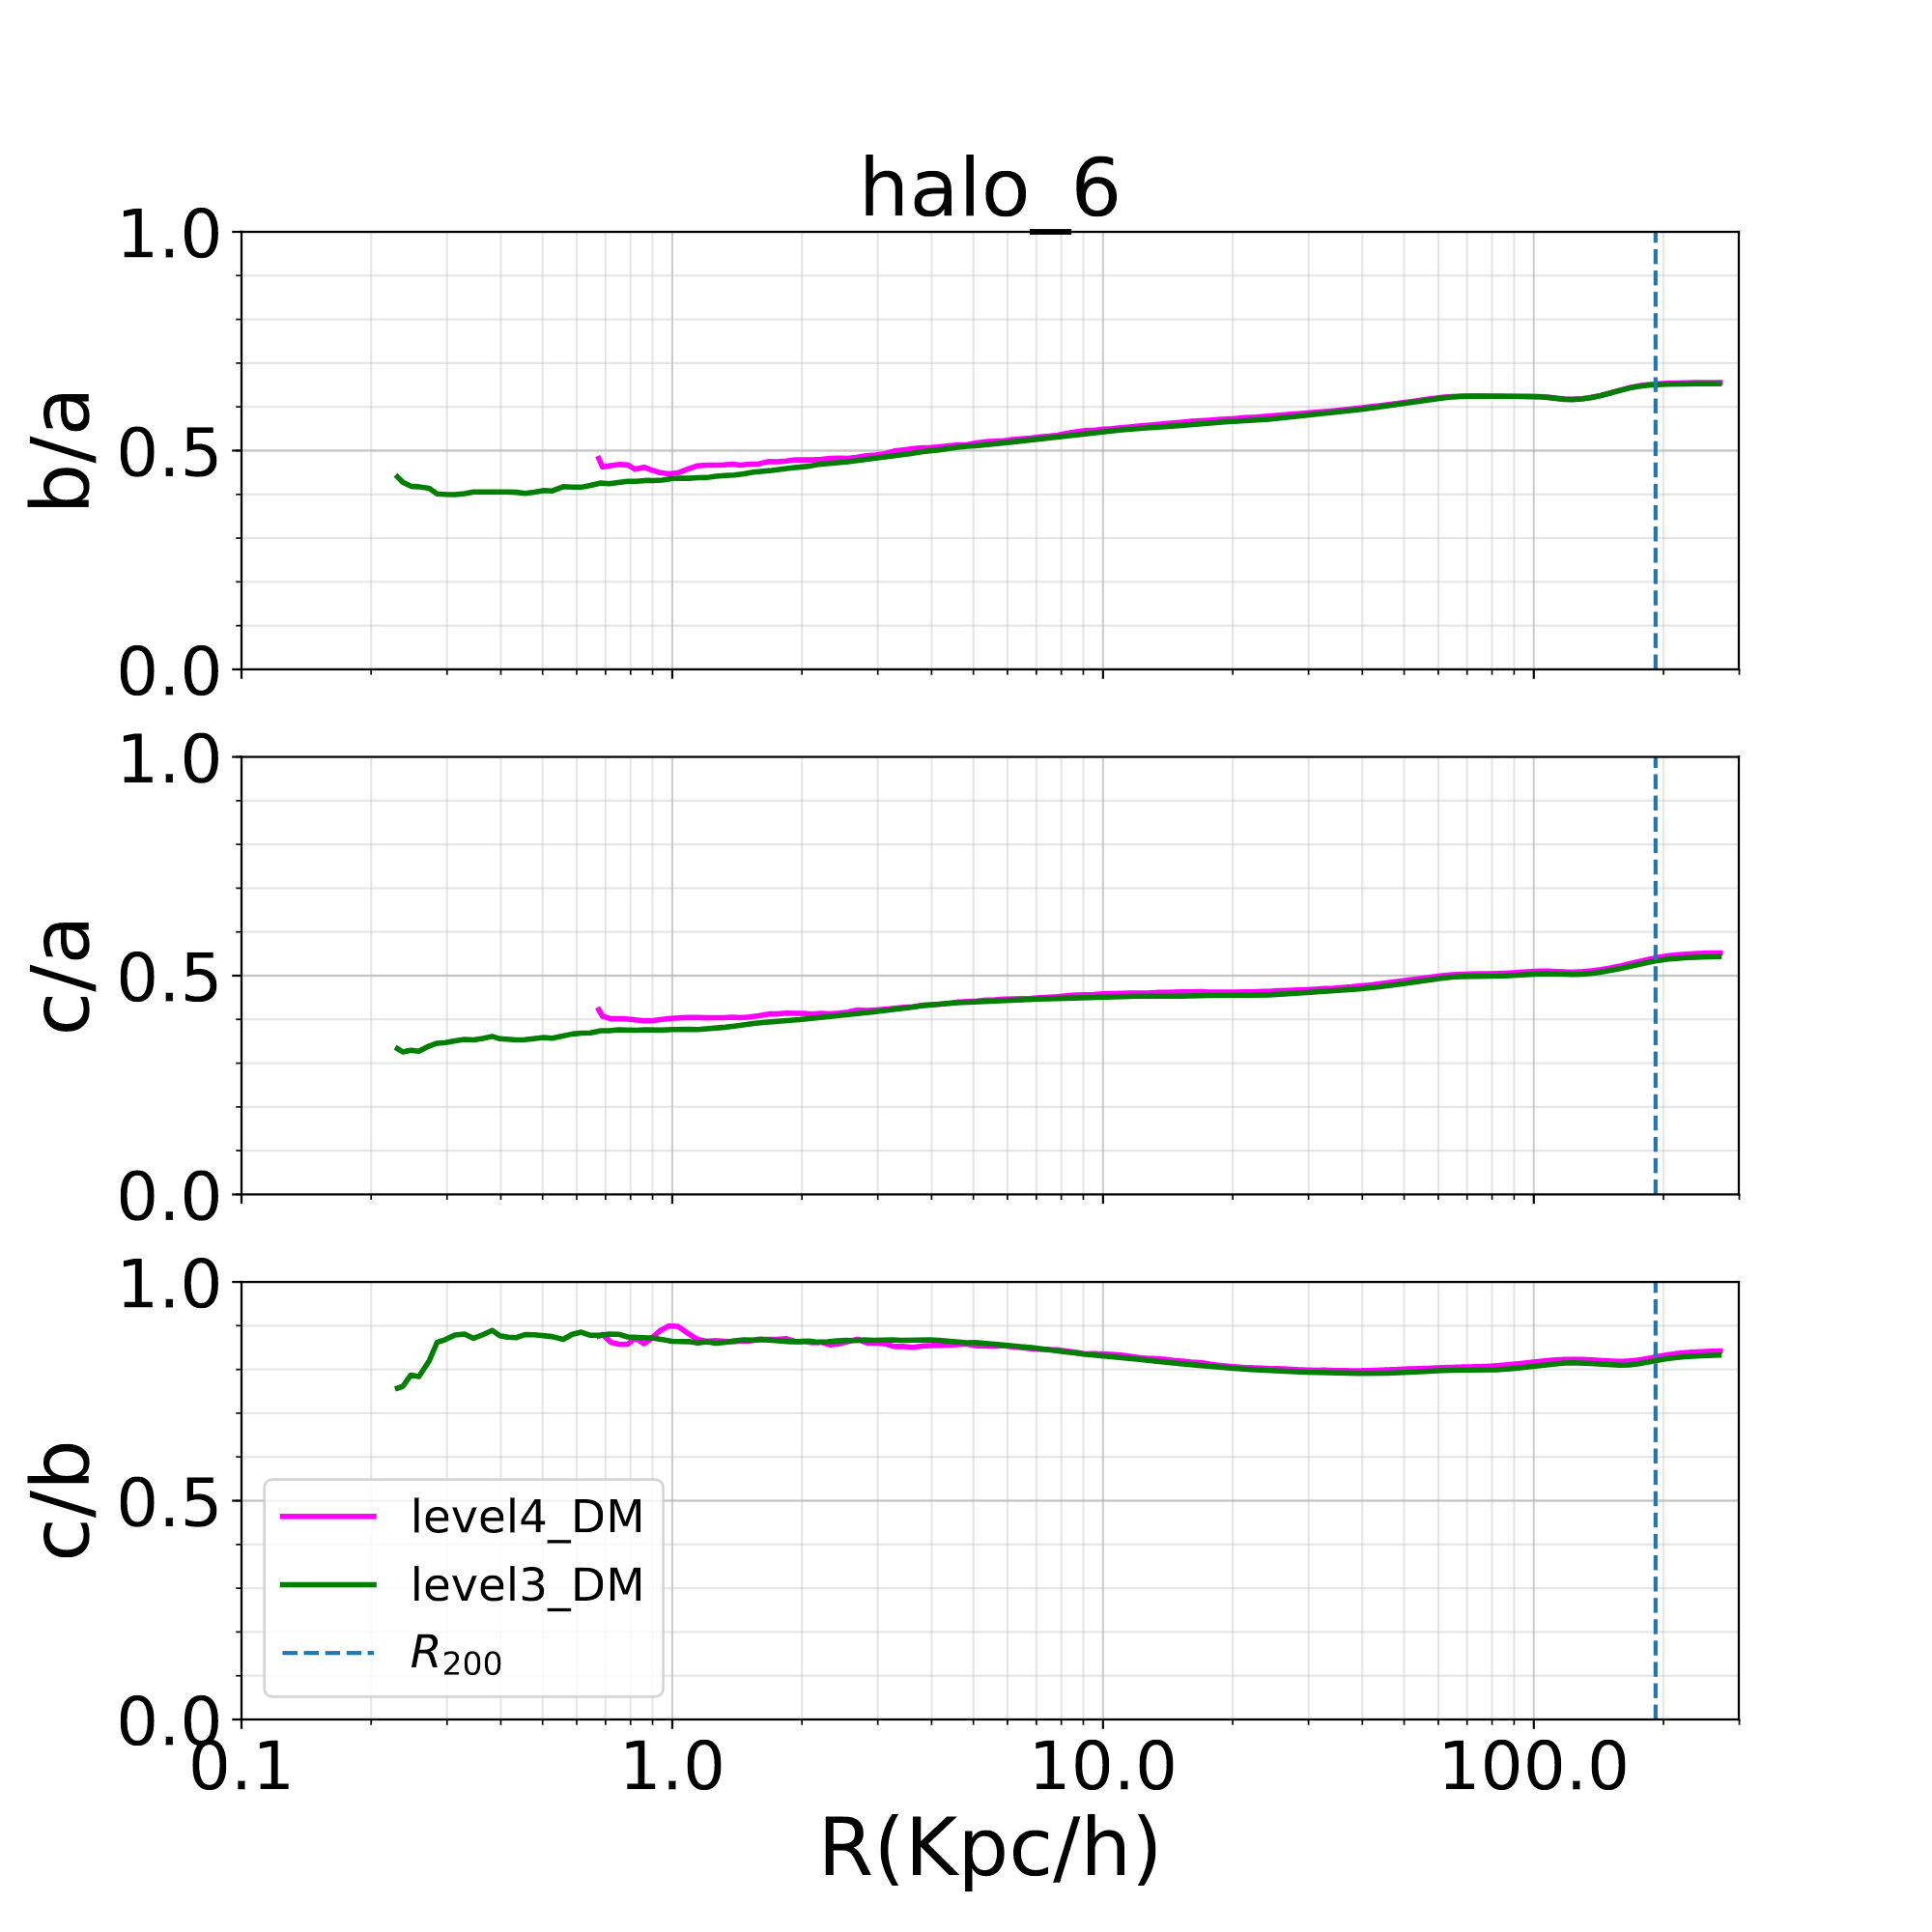
\includegraphics[width=0.7\columnwidth]{./pics/Convergence/halo6_DM_3Vs4_good.png}}
  \hfill
  \subfloat[halo 27 MHD]{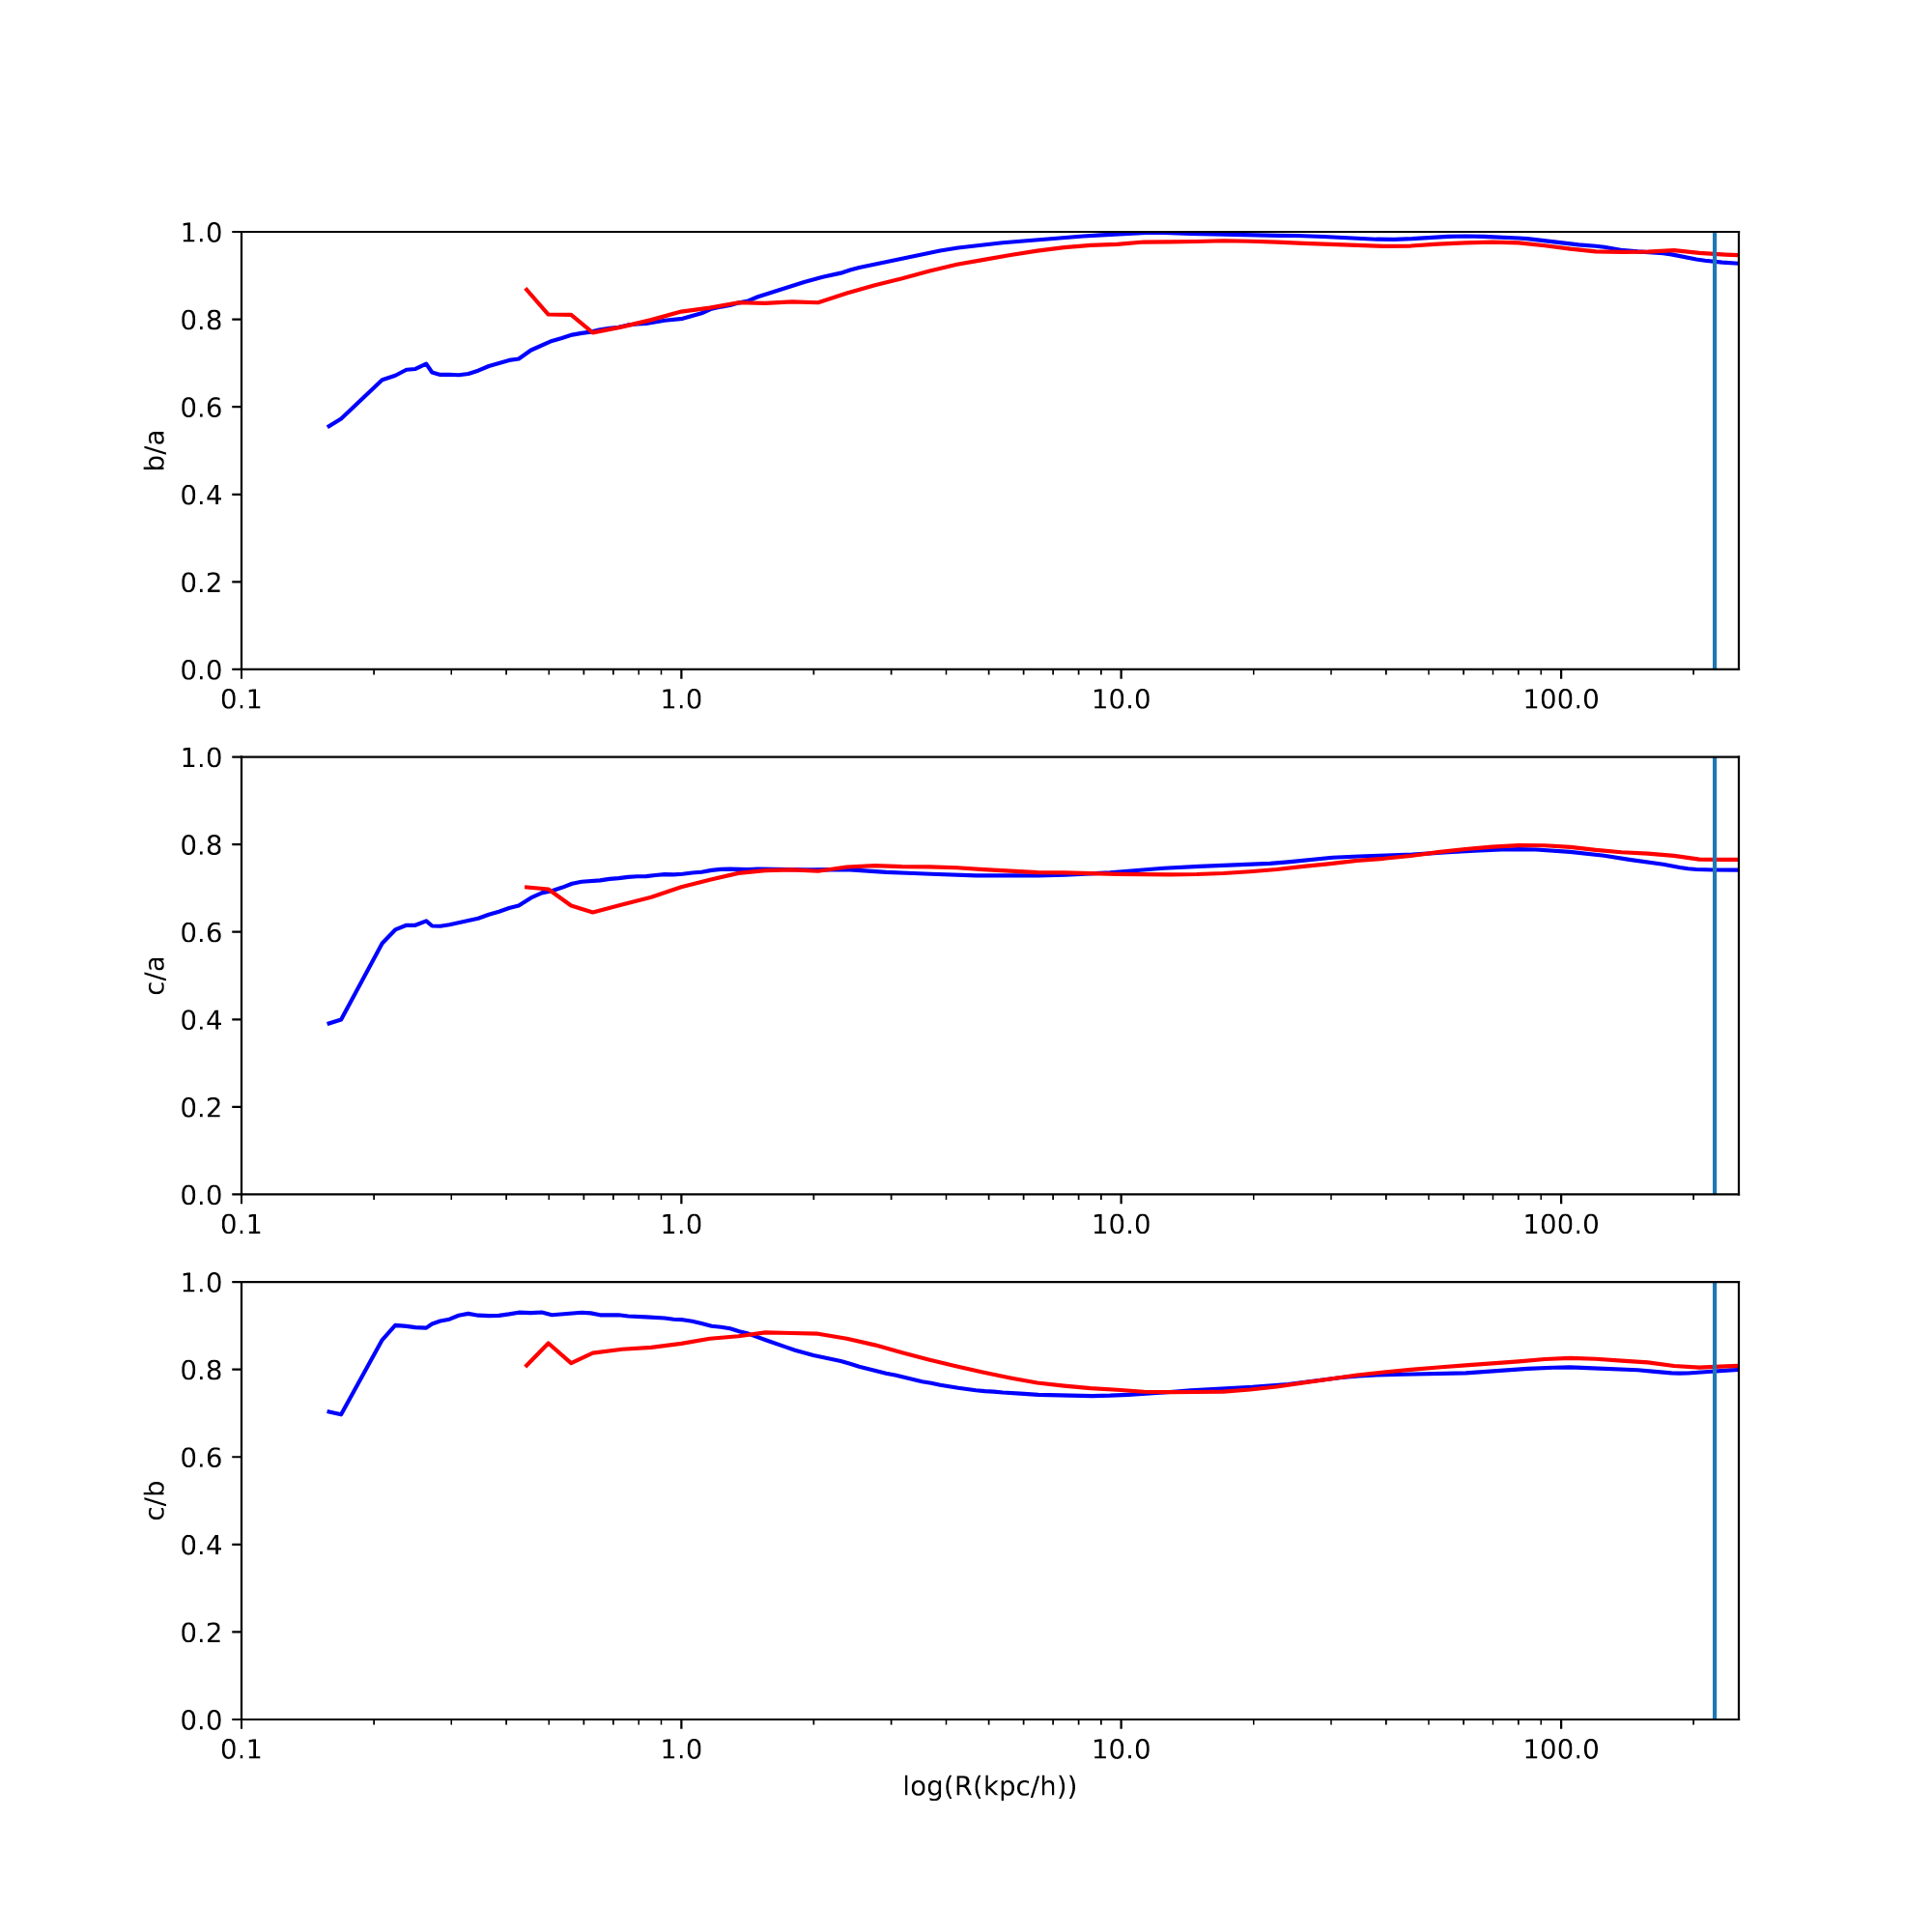
\includegraphics[width=0.7\columnwidth]{./pics/Convergence/halo27_MHD_3Vs4_good.png}}
  \caption{Examples of halos where level 3 (pink) and level 4 (green) calculations are in good agreement.}
  \label{fig:goodConvergence}
\end{figure}



\begin{figure}[!ht]
  \centering
  \subfloat[halo 16 DM]{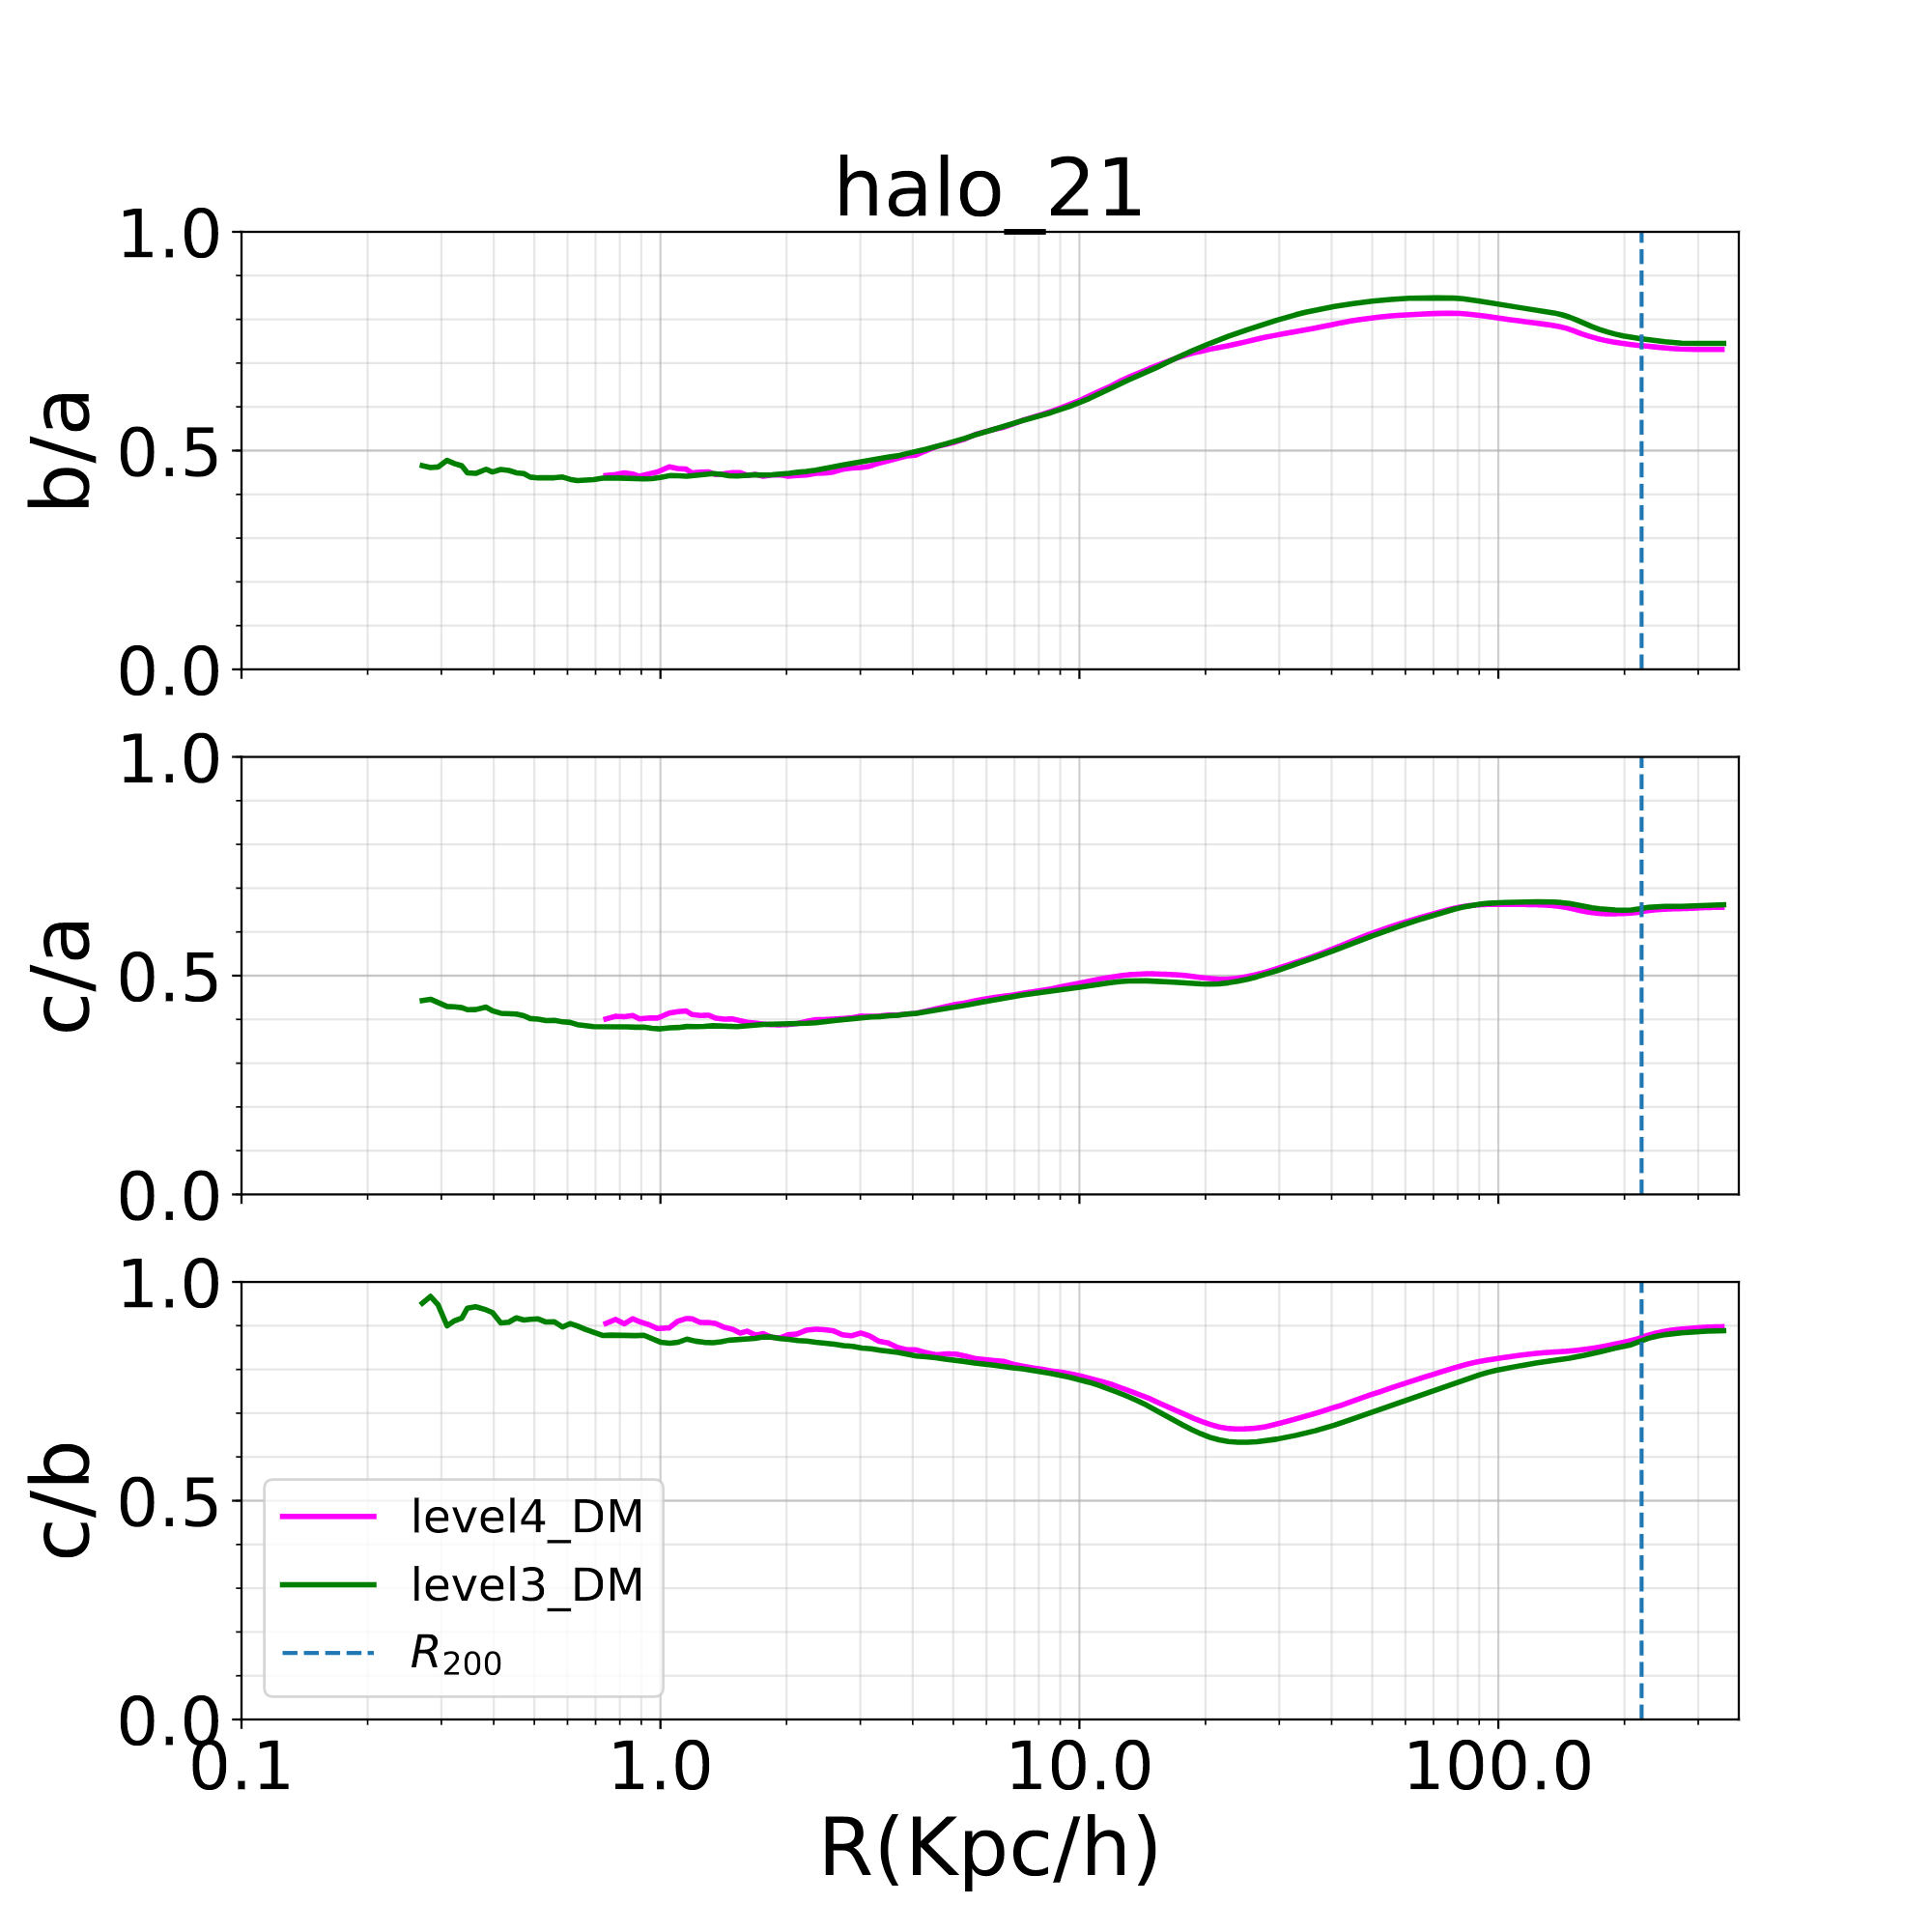
\includegraphics[width=0.8\textwidth]{./pics/Convergence/halo21_DM_3Vs4_bad.png}}
  \hfill%\hspace{-0.5em}
  \subfloat[halo 23 MHD]{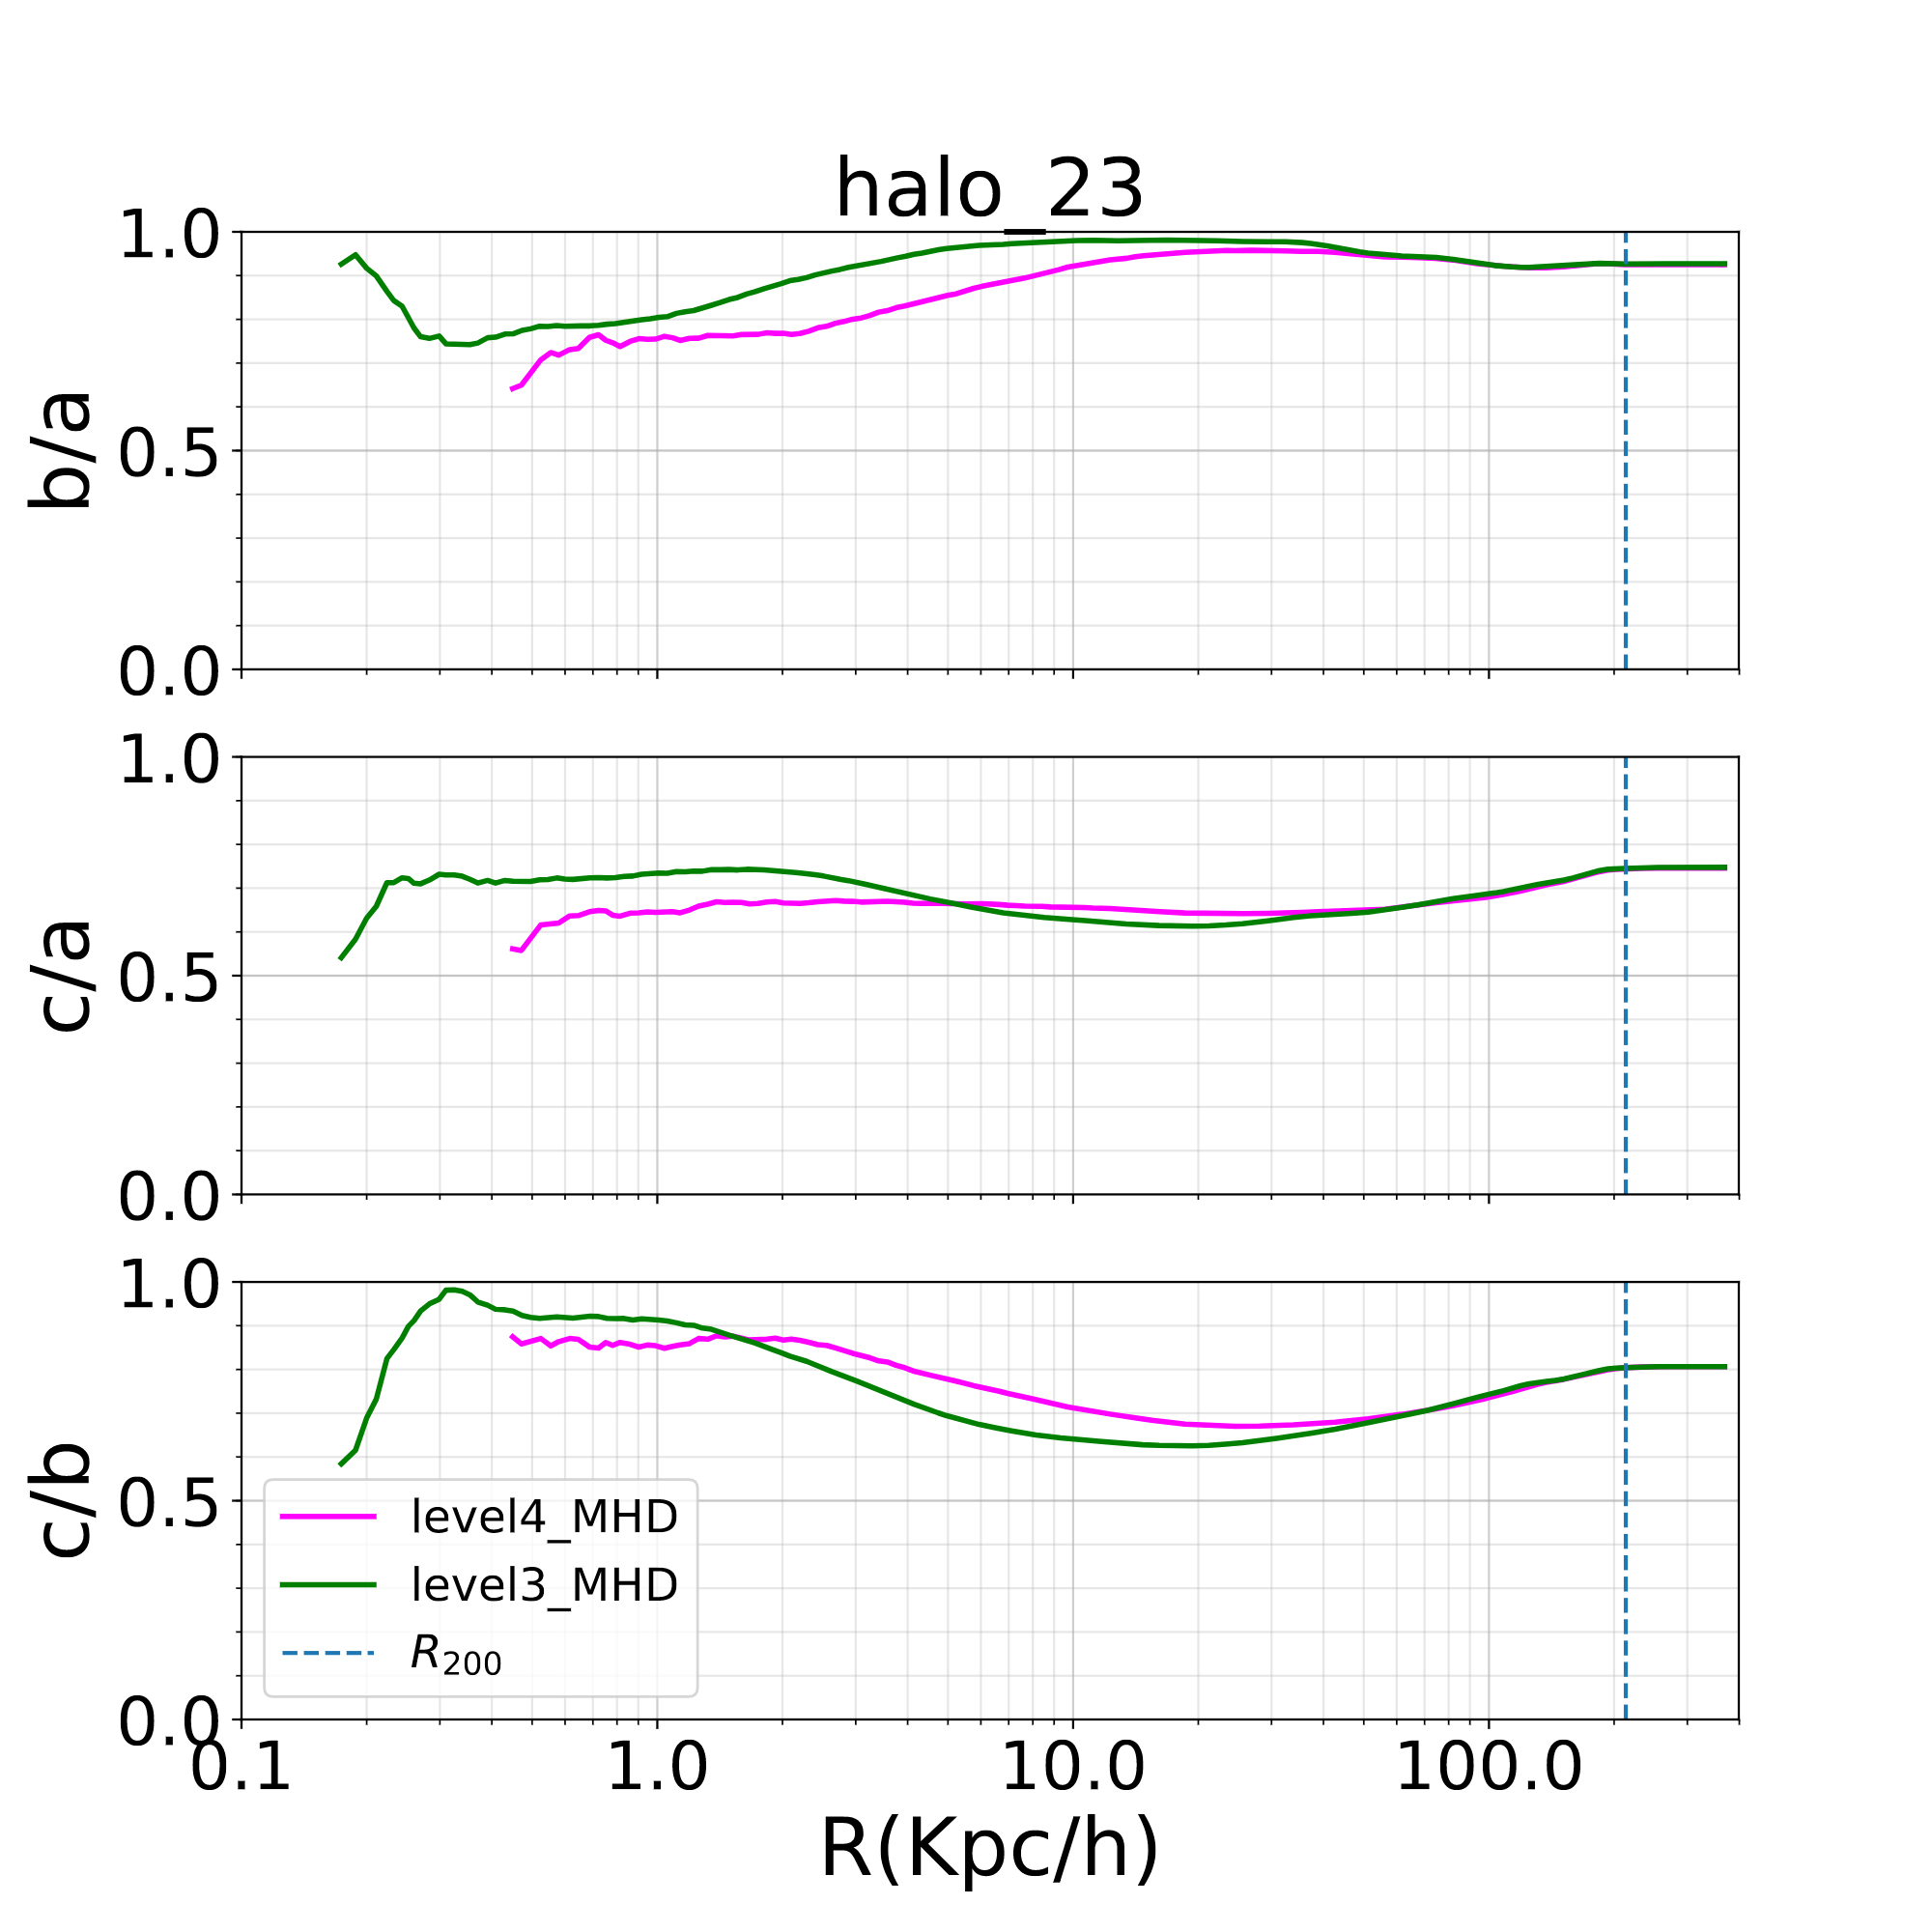
\includegraphics[width=0.8\textwidth]{./pics/Convergence/halo23_MHD_3Vs4_bad.png}}
  \caption{Examples of halos that have an appreciable difference between level 3 (pink) and level 4 (green) calculations. }
  \label{fig:badConvergence}
\end{figure}


For instance, by simple inspection, we notice that there is no apparent systematic way in which resolution affects the halo shape. That is, sometimes the halo appears rounder and some times it is affected towards a more triaxial shape. This is important for our study as we focus our efforts on the analysis of the triaxial properties of the halo. Incidentally, the DM-only halos remain unchanged with the exemption of the radial regimes where the number of particles naturally affects our shape-calculating method. However, for MHD simulations, the resolution of gas influences the measurement not only in the inner parts, where discretization issues are evident, but it has a more global effect. We suspect this is caused by the scattering of particles due to dense structures formed by gas, whose effect is affected by resolution. Nevertheless, further calculations need to be performed to confirm if these resolution biases are directly caused by AllGood's method for calculating shapes, or are caused because structures are indeed affected by numerical errors from the solution of fluid equations of matter.\\

Consequently, we decided to isolate the few-particle effect on our shape calculations without recurring to the less-resoluted simulations of level 4. Taking into account that the resolution difference between level 3 and level 4 simulations is a factor of 8 in the number of DM particles, we randomly selected particles from level 3 halos at redshift 0 to produce 10 samples of approximately the same size as level 4 simulations. We then proceeded to analyze the effect of lowering the number of particles on the calculated shape of the halo. In figures \ref{fig:convergence} we ploted the original level 3 shapes as well as the 10 level 3 samples. For each radius, we calculated the standard deviation of the sample shape and illustrated 3-sigma range to compare with the respective level 4 shape values.\\  

From the graphics on \ref{fig:convergence}, it is clear that the plotted fractional difference is not actually big and remains under $1\%$ for the majority of the radial profile. It becomes important for radii less than $1Kpc$ due to the lack of particles for approximating an elliptical shape shape. This is corroborated by the $3\sigma$ range, which also becomes evident around $1Kpc$. We then deduce from this convergence analysis that for radii bigger than $1Kpc$, the differences of level 3 and level 4 ellipses cannot be explained as an effect of the lack of particles. This is a confirmation that all kinds of matter are directly affected by resolution due to precision-sensitive events on the history of formation or because the numerically calculated gravitational potential of matter itself is affected and continuously influences surrounding structures. Either way, even for the most resolution-biased cases, we can say that for the purposes of this study, convergence is achieved to a reasonable extent.\\  

\begin{figure}[!ht]
  \centering
  \subfloat[halo 24 MHD]{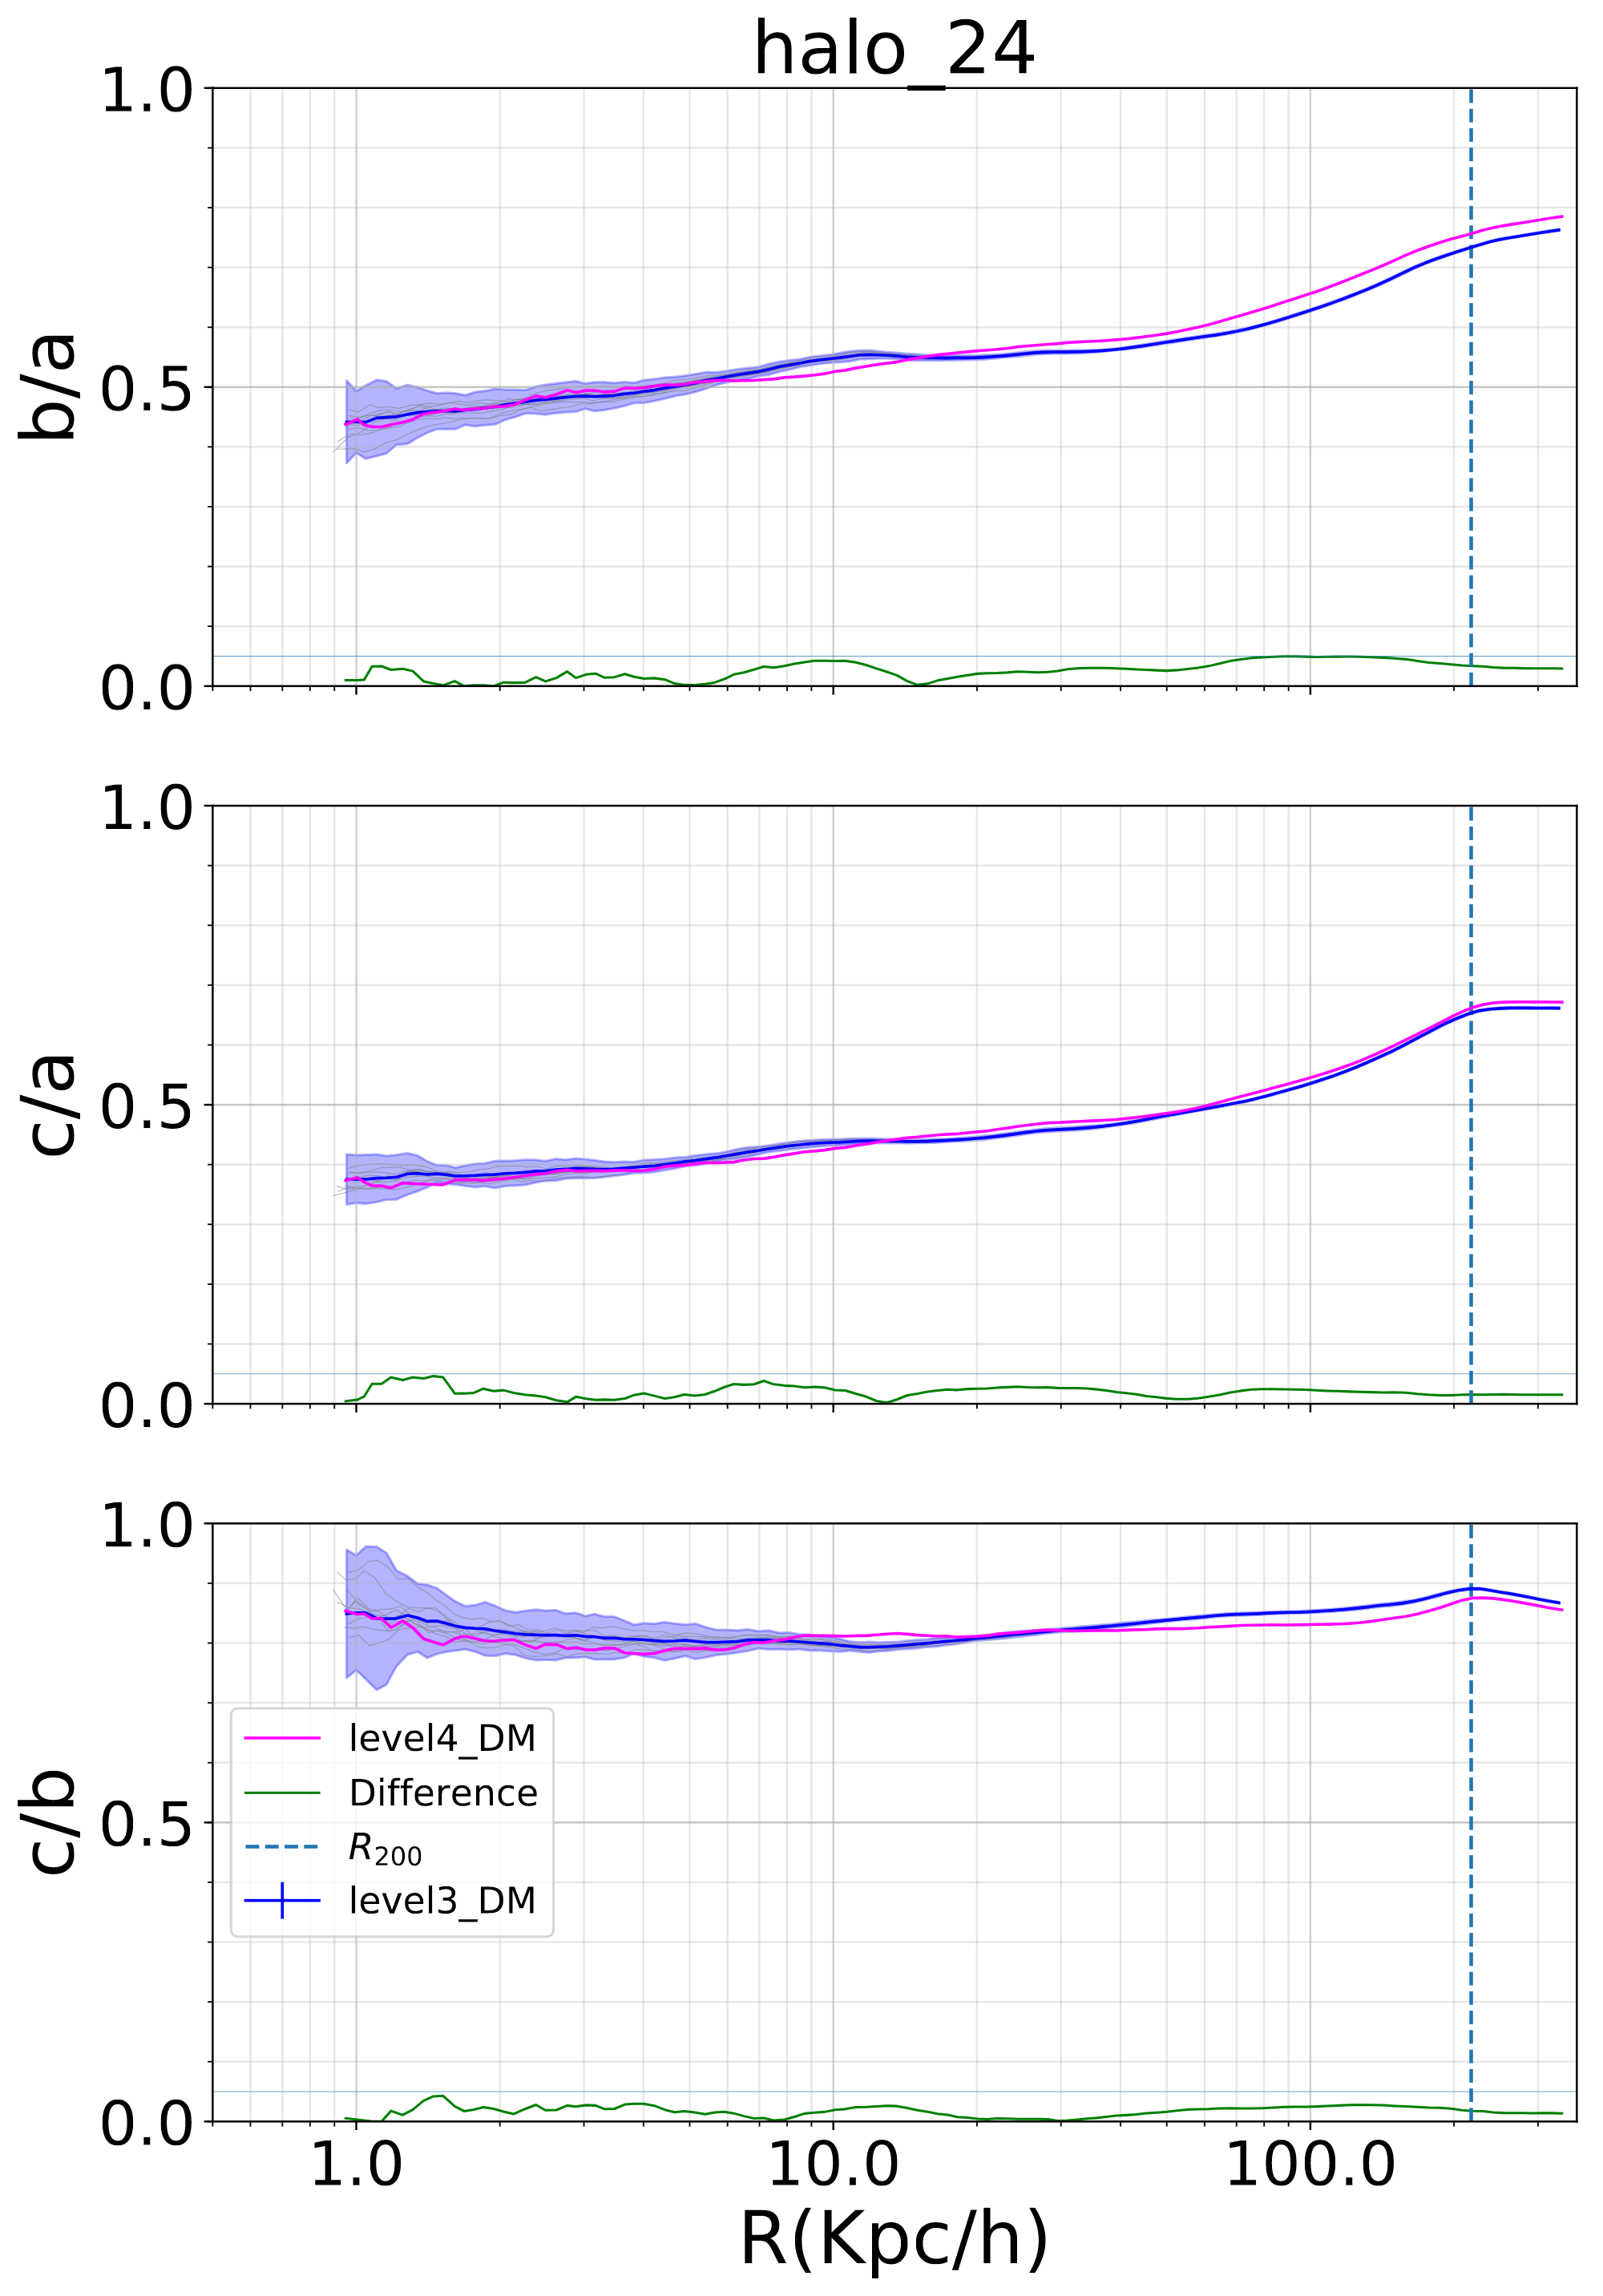
\includegraphics[width=0.7\columnwidth]{./pics/Convergence/rand_conv_halo24_DM.png}}
  \hfill
  \subfloat[halo 24 DM]{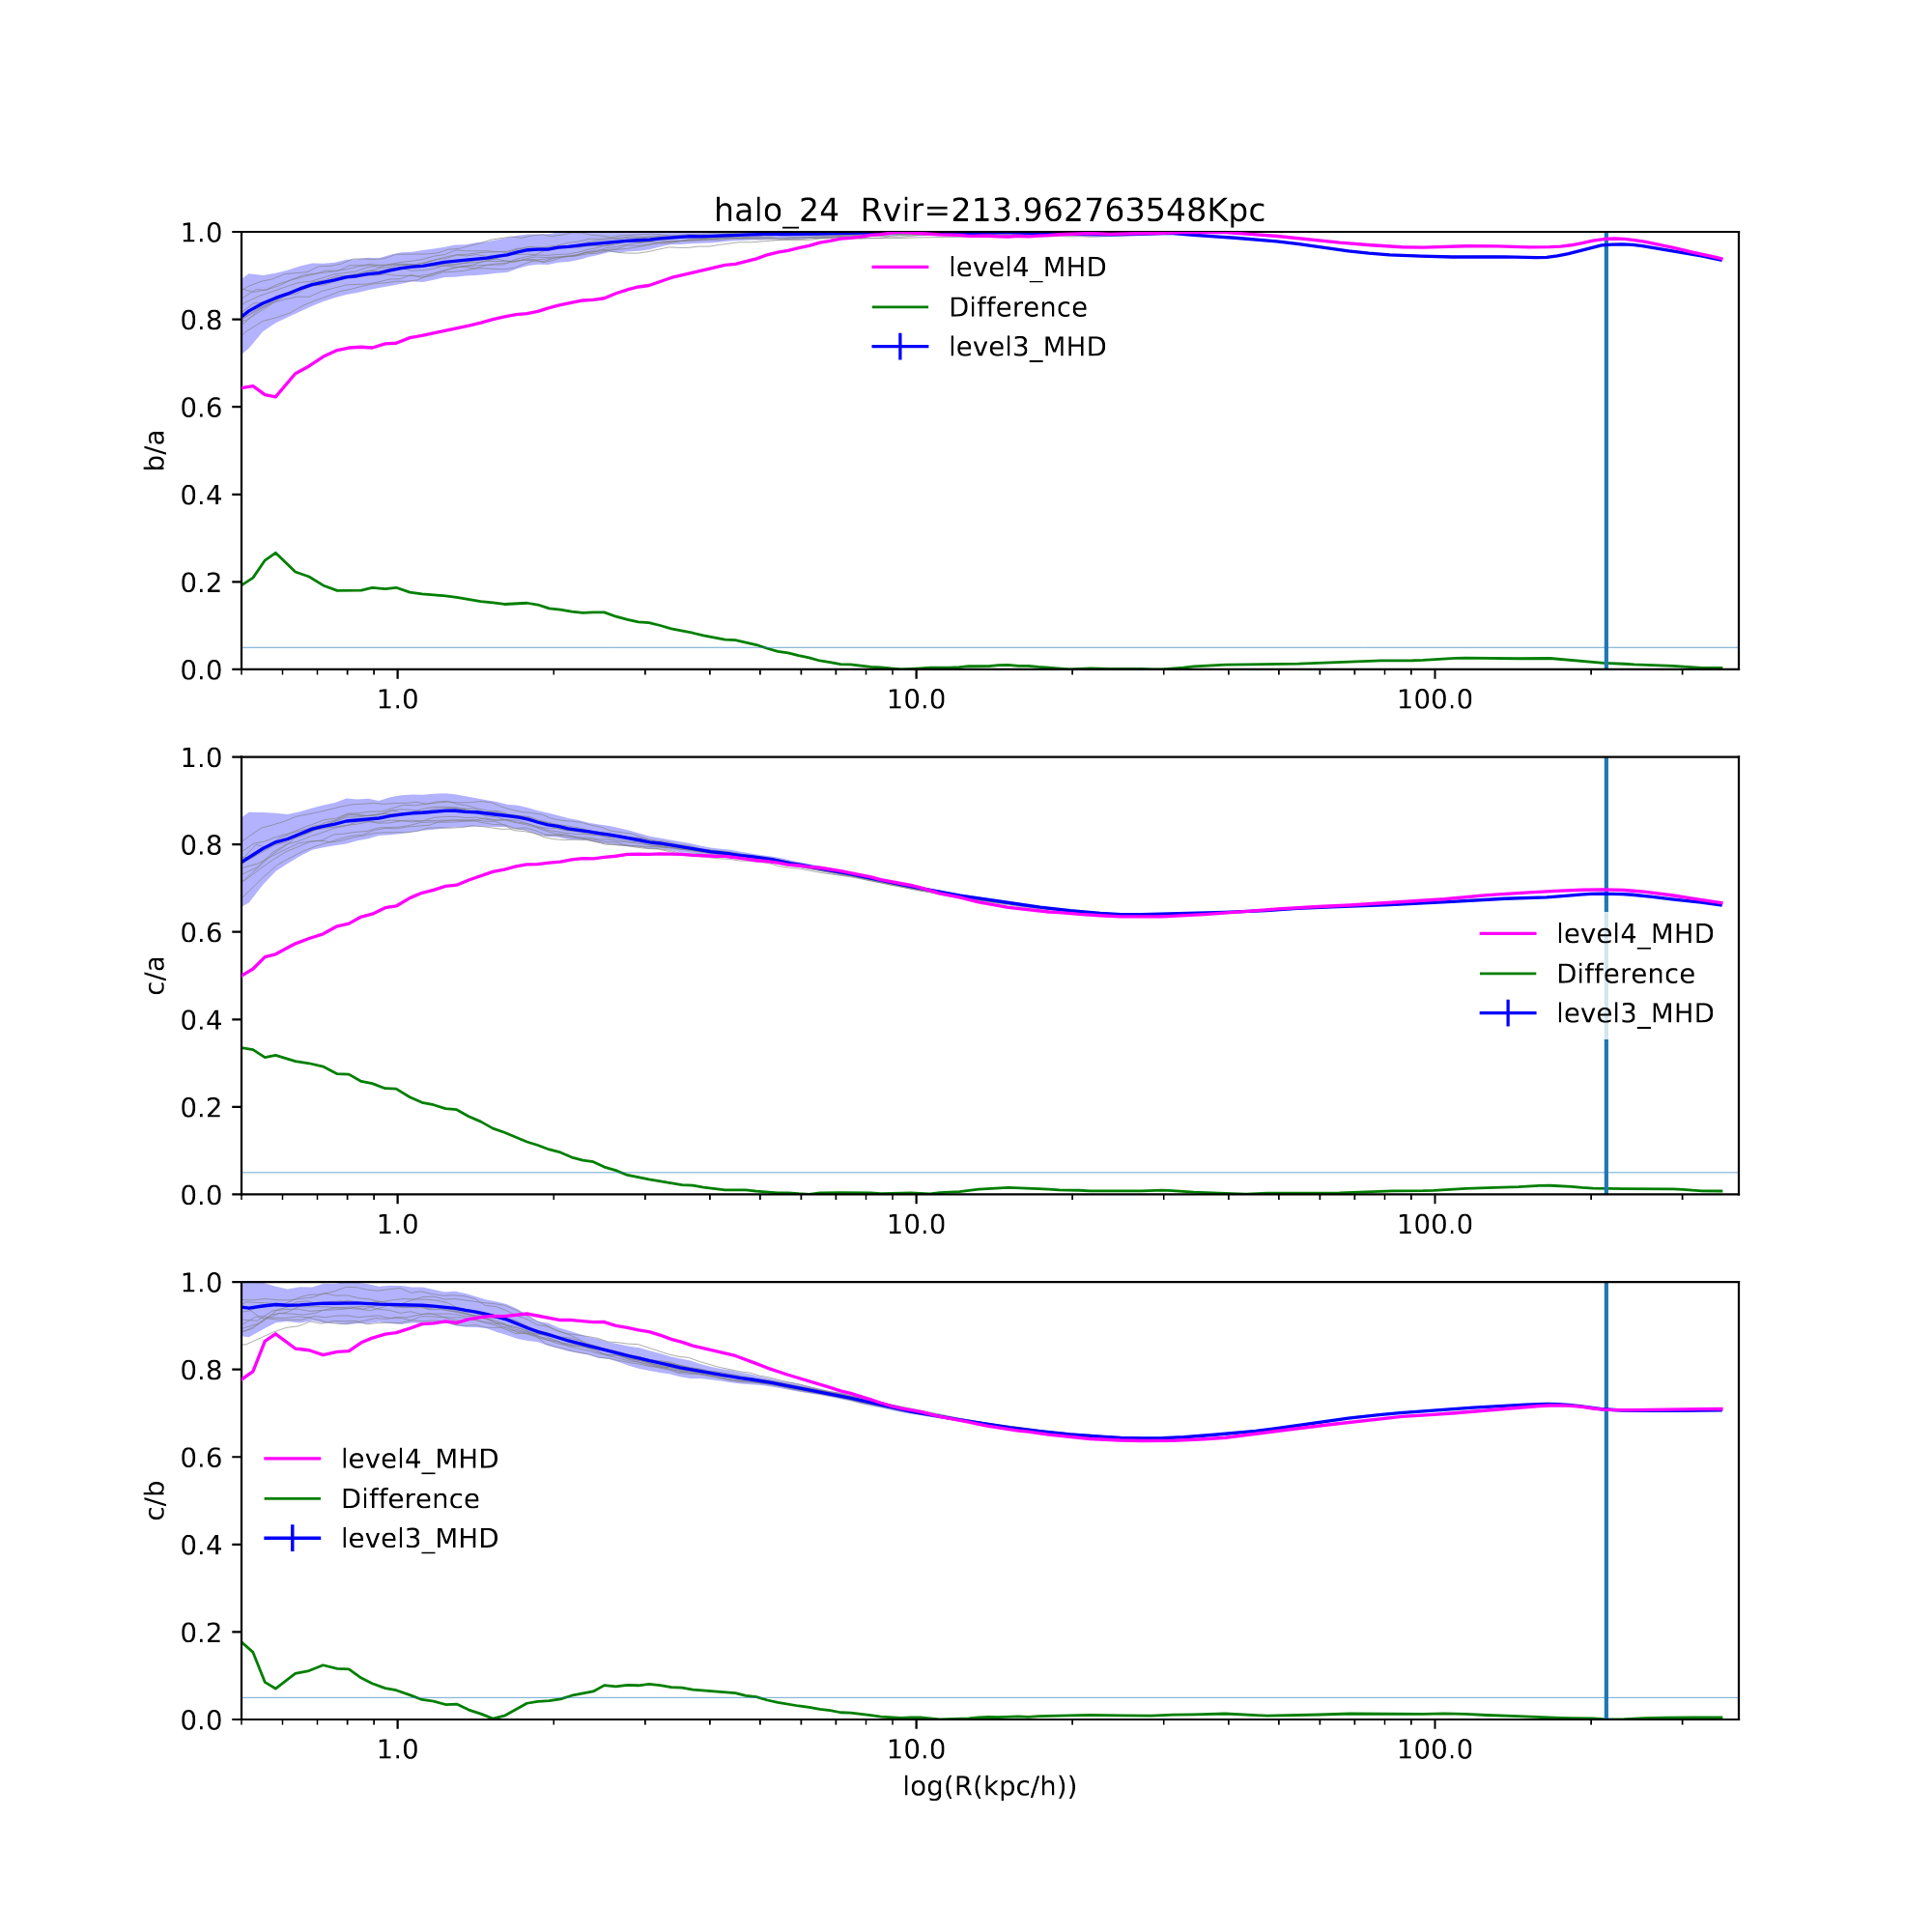
\includegraphics[width=0.7\columnwidth]{./pics/Convergence/rand_conv_halo24_MHD.png}}
  \caption{Comparison of the effect of resolution on DM and MHD simualations. Here level4 curves (magenta) are compared to the mean and 2std (confirm) of the random-sampled curves from level3. For better comparison of the effect of resolution, the difference percent is plotted in green.}
  \label{fig:convergence}  
\end{figure}

\section{The shape's radial dependence}
One of the first results we obtained in this study is related to the evolution of the DM halo shape in terms of the radius at which it is sampled. We already expect from previous work that the shape does not remain constant along the radius \cite{Vera-Ciro et al 2011}. Specifically, we know that halos are gradually constructed from inner shells to outer shells through the accretion of matter from cosmic structures \cite{}. Inner shells are shielded from the gravitational potential from outter regions as a consequence of the Gauss law. Therefore, inner shells tend to conserve their shape. Outter shells, on the other side, are affected by the increasing gravitational potential form the inside of the halo, which makes them prone to scattering effects. This scattering of particles has a "rounding" effect on the outerskirts shape. For this reason, we expect on both simulations (MHD and DM) that halos are more triaxial on inner regions and more spherical at bigger radii. This effect has been corroborated on multiple cosmological simulations (Citas)\cite{}. \\


\begin{figure}[!ht]
  \centering
  \subfloat[halo 27 DM shape at small radius]{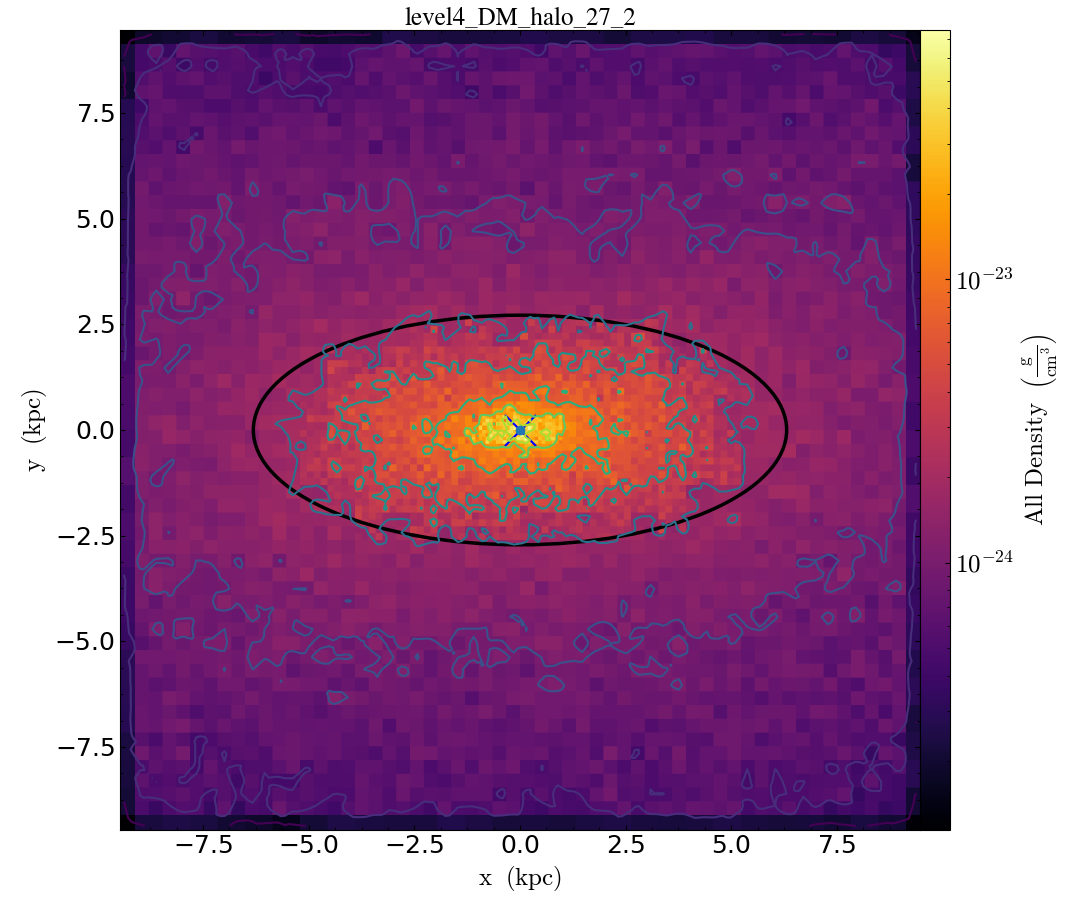
\includegraphics[width=0.5\columnwidth]{./pics/MHD_Vs_DM/level4_DM_halo_27_inner.png}}
  \hfill
  \subfloat[halo 27 DM shape at big radius]{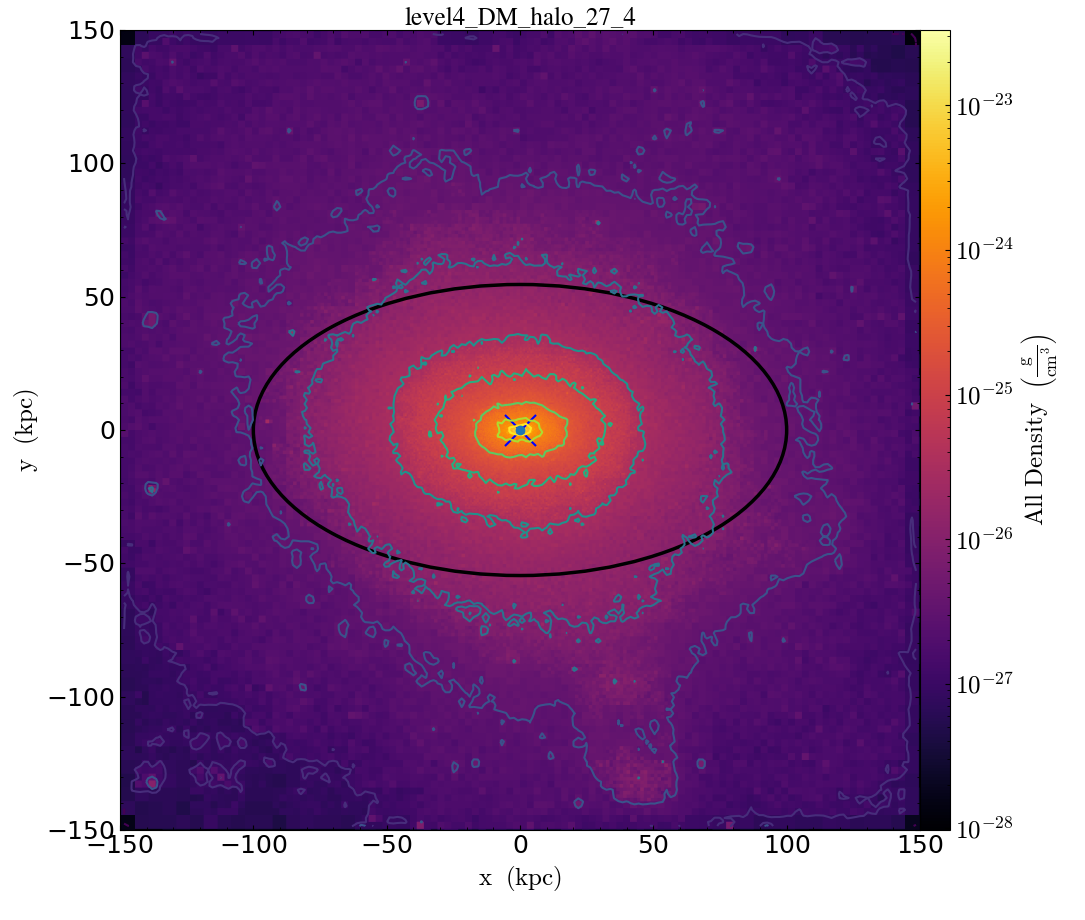
\includegraphics[width=0.5\columnwidth]{./pics/MHD_Vs_DM/level4_DM_halo_27_outter.png}}
  \hfill
  \subfloat[halo 27 MHD shape at small radius]{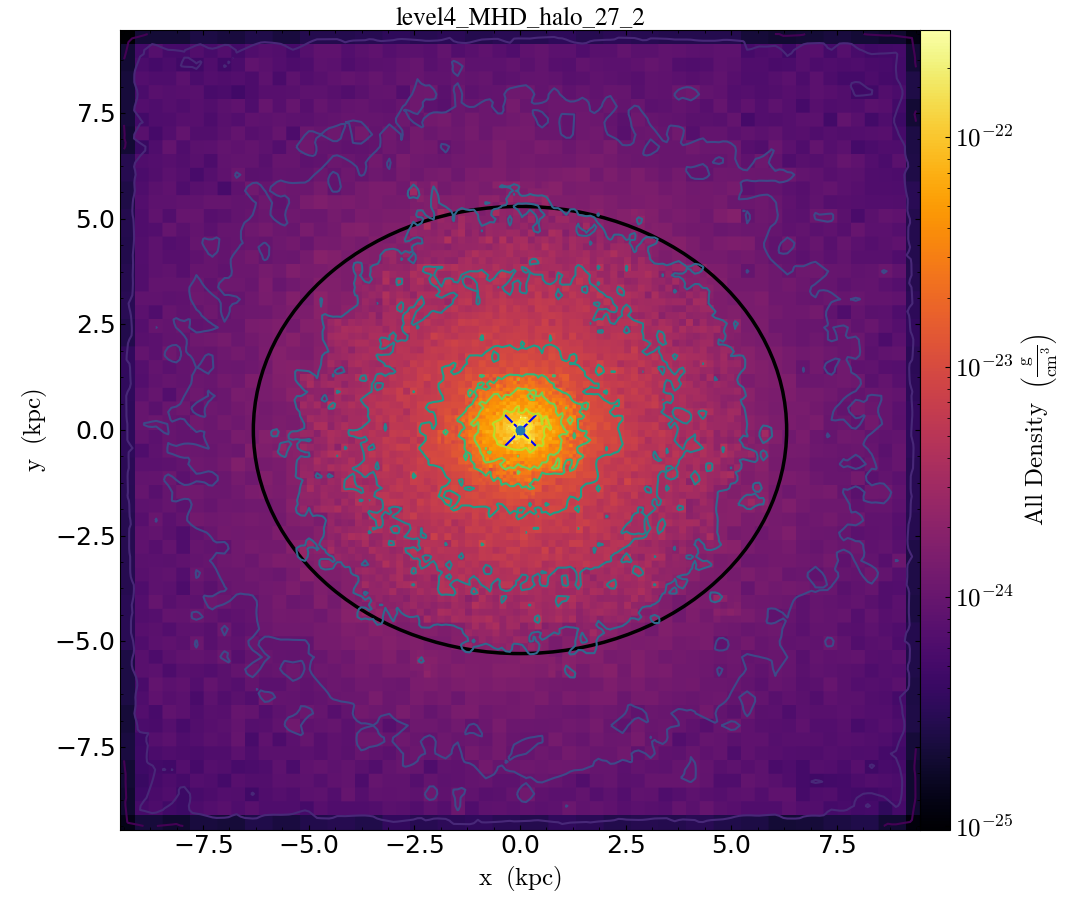
\includegraphics[width=0.5\columnwidth]{./pics/MHD_Vs_DM/level4_MHD_halo_27_inner.png}}
  \hfill
  \subfloat[halo 27 MHD shape at big radius]{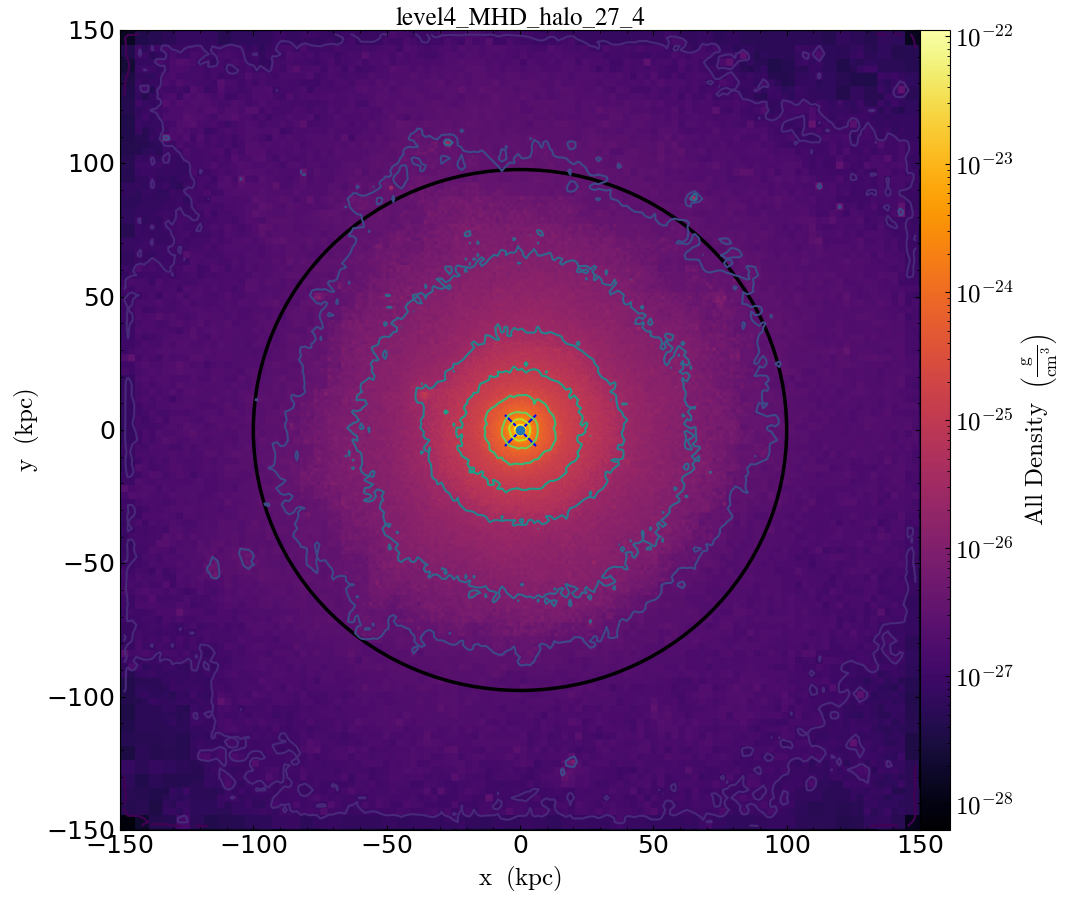
\includegraphics[width=0.5\columnwidth]{./pics/MHD_Vs_DM/level4_MHD_halo_27_outter.png}}
  \caption{Example of the dependence of shape in terms of the radius. All graphics have matching orientation (which may not be the same) with their respective principal axes at the shown radii. The horizontal and vertical axes are aligned to the major and medium semi-axes respectively. }
  \label{fig:slices}
\end{figure}

In figures \ref{fig:slices}, we present a halo in which the rounding effect is specially evident for both degrees of realism (Horizontal comparison). However, to eliminate any possible cualitative bias, we present a more detailed and quantitative version of this effect in terms of the radius on figure \ref{fig:DM_MHD}. There, we include all axial ratios, which clearly become closer to 1 (more spherical) for bigger radii. Besides the axial ratios, we included a quantification of the triaxiality, namely $T=\frac{1-b/a}{1-c/a}$.\\

 This measurement $T$ tends towards unity when the medium-to-major axis ratio becomes equal to the minor-to-major ratio, i.e. when the halo becomes prolate. In the case where the medium axis is very close to the major axis, having a different minor axis, $T$ tends to a null value, i.e. when the halo tends to a oblate shape. In these terms, halos are expected to be more prolate on the inside and more oblate on the outside. Even though the perfect spherical shape has a divergent/undefined $T$ value, prolate shapes are associated with triaxial characterizations and oblate shapes are identified as approximately spherical shapes. This, however, can be confirmed on the triaxiality plane where we can also demonstrate that this is in fact a global tendency on all halos.\\


\begin{figure}
\centering
{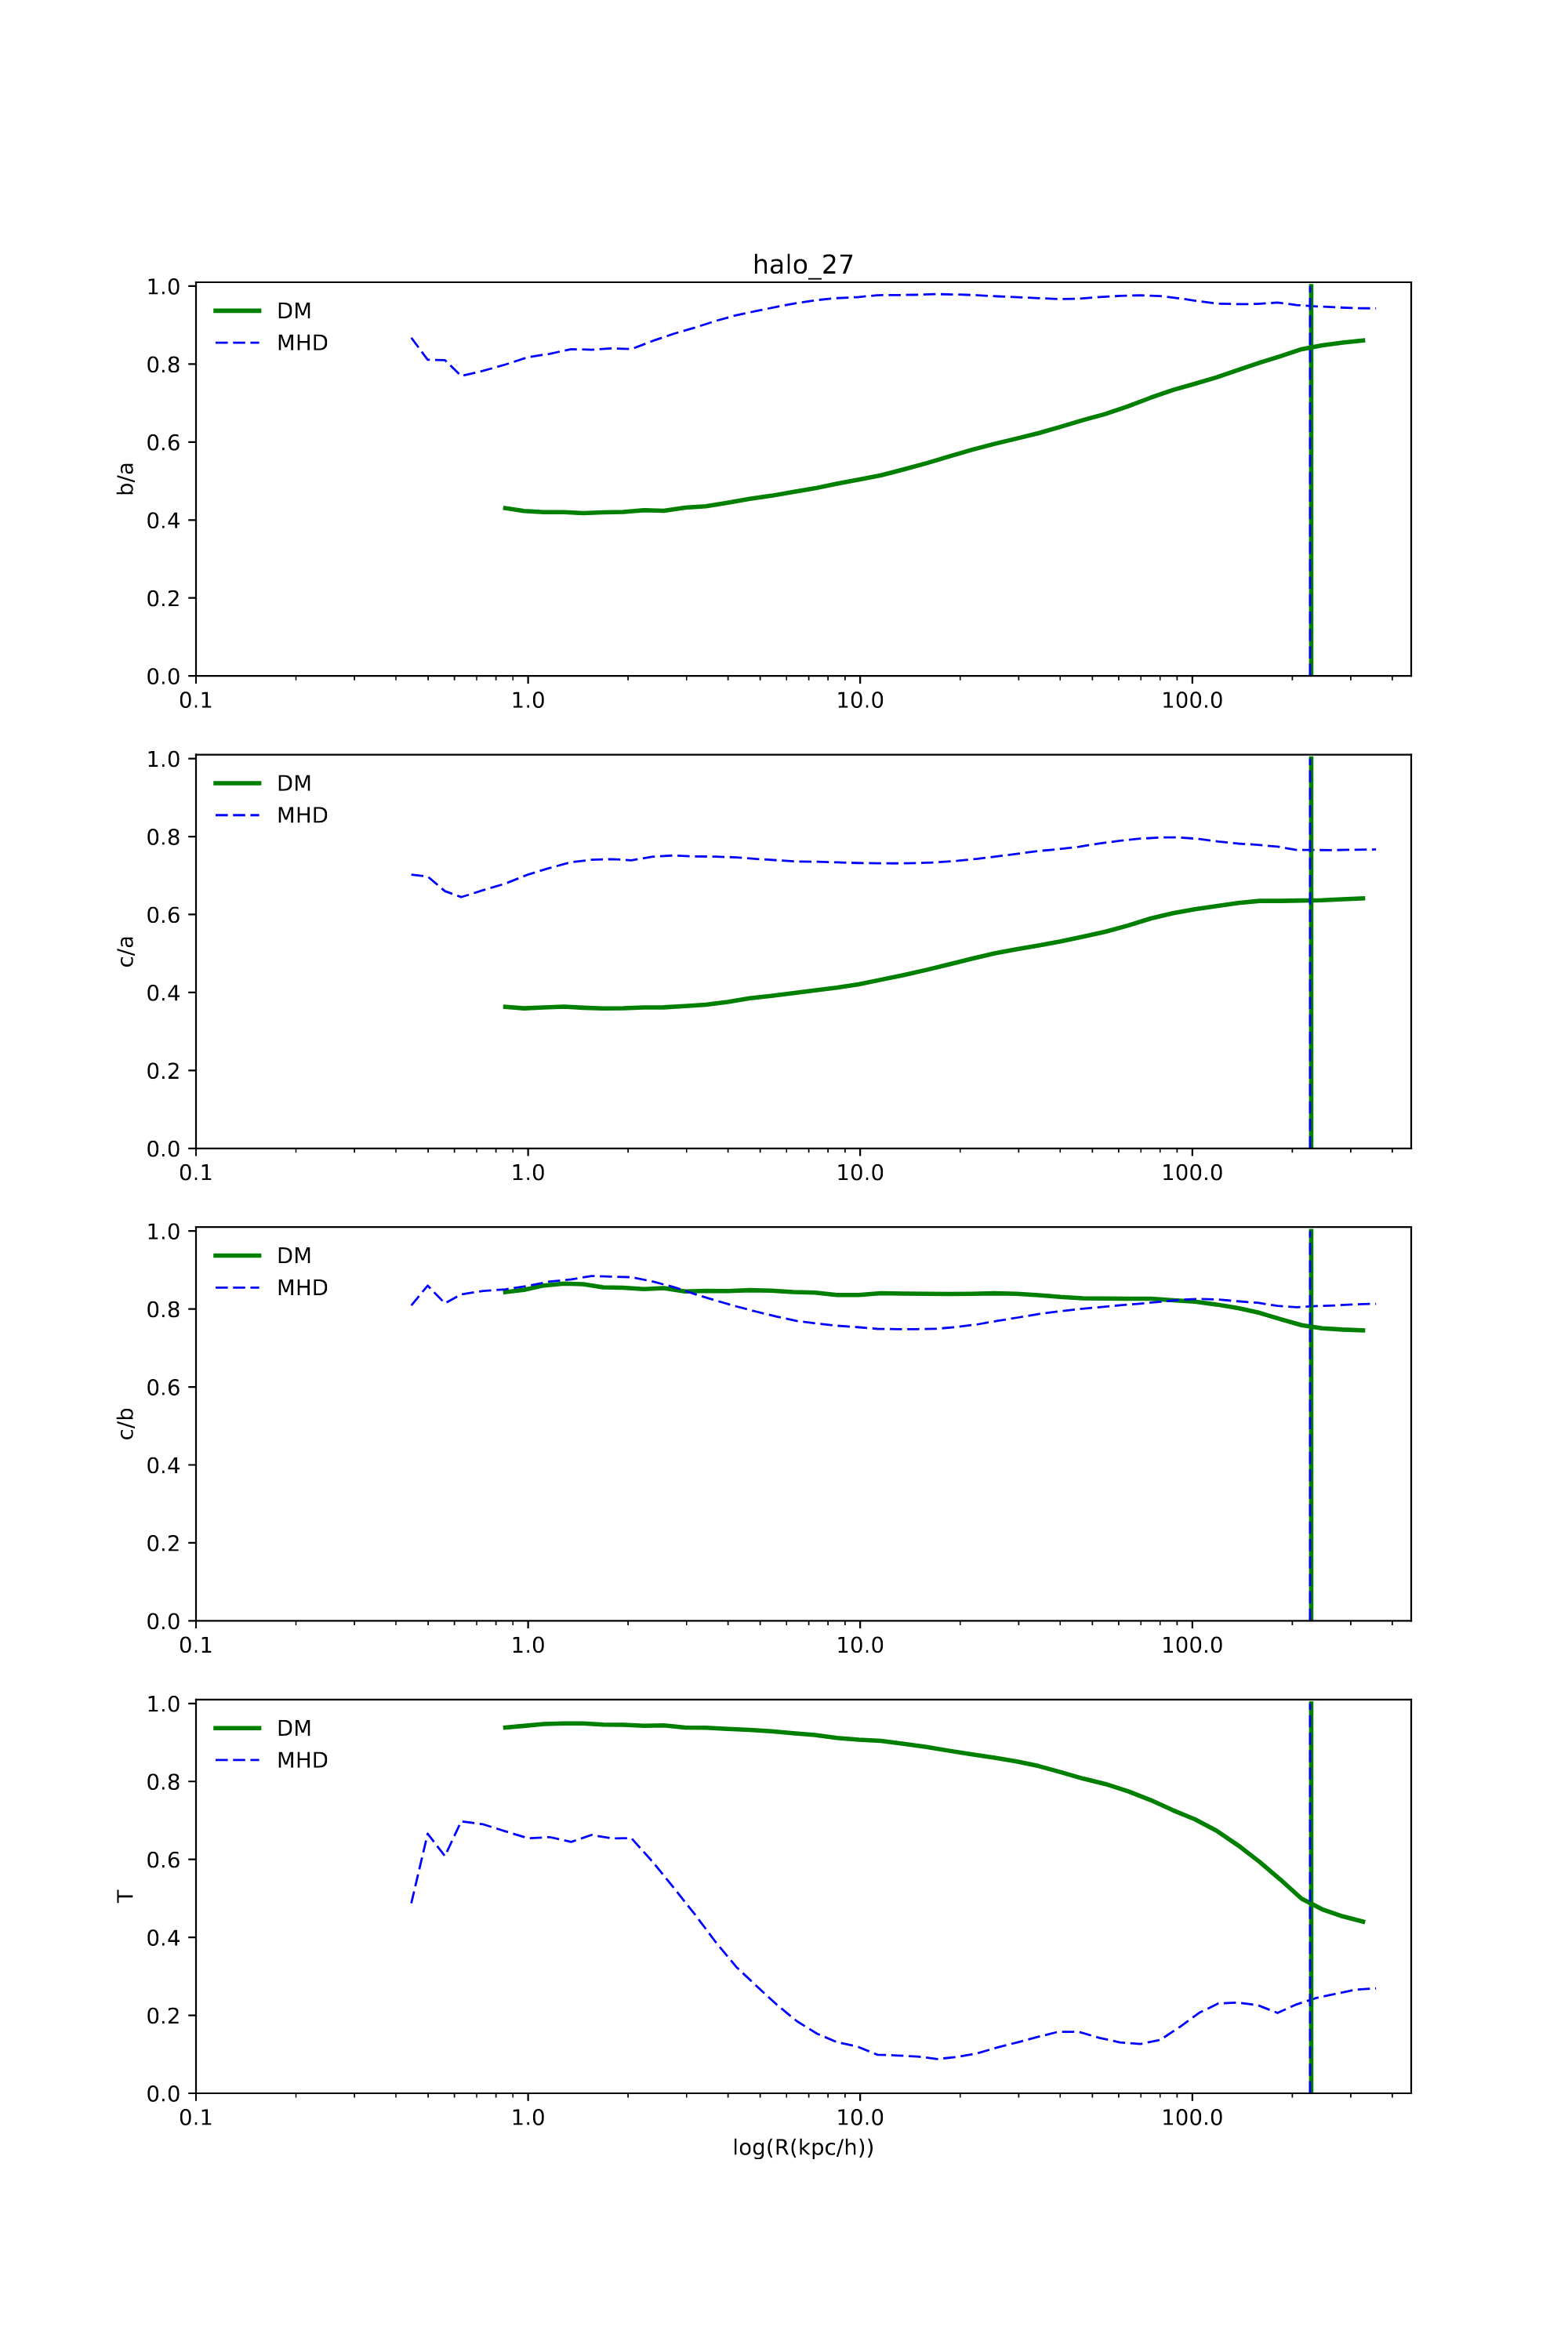
\includegraphics[width=1\columnwidth]{./pics/MHD_Vs_DM/level4_halo_27_DM_Vs_MHD.png}}
\caption{Semi-axial ratios and triaxiality $\frac{1-b/a}{1-c/a}$ as function of radius for semi-axes $a\geq b\geq c$. The MHD simulation (blue dotted line) shows ratios closer to $1$ than those from the DM-only (green solid line) simulation. The rounding effect with radius for each simulation separatedly is also well-appreciable in this graphic. The radial-rounding, as well as the gas-presence amplification can be evidenced on the triaxiality function. }
\label{fig:DM_MHD}
\end{figure} 


In figure \ref{fig:Triaxiality_Inner_Outer}, we show the axial ratios on the plane $c/a Vs b/a$. There, each dot represents a specific halo shape at a specific radius. In this plane, oblate halos are represented by the vertical line $x = 1$, prolate halos are identified on the identity line and spheres are exactly the point $(1,1)$. This gives us a broader idea of the evolution of the shape than a single number $T$. In this figure, the tendency is clear for DM and MHD halos to get rounder with increasing radius. In fact, the difference in shape clear enough that it is possible to identify groups in case the radius label is lost.\\

\begin{figure}[!ht]
  \centering
  \subfloat[Level4 MHD Vs DM at inner regions]{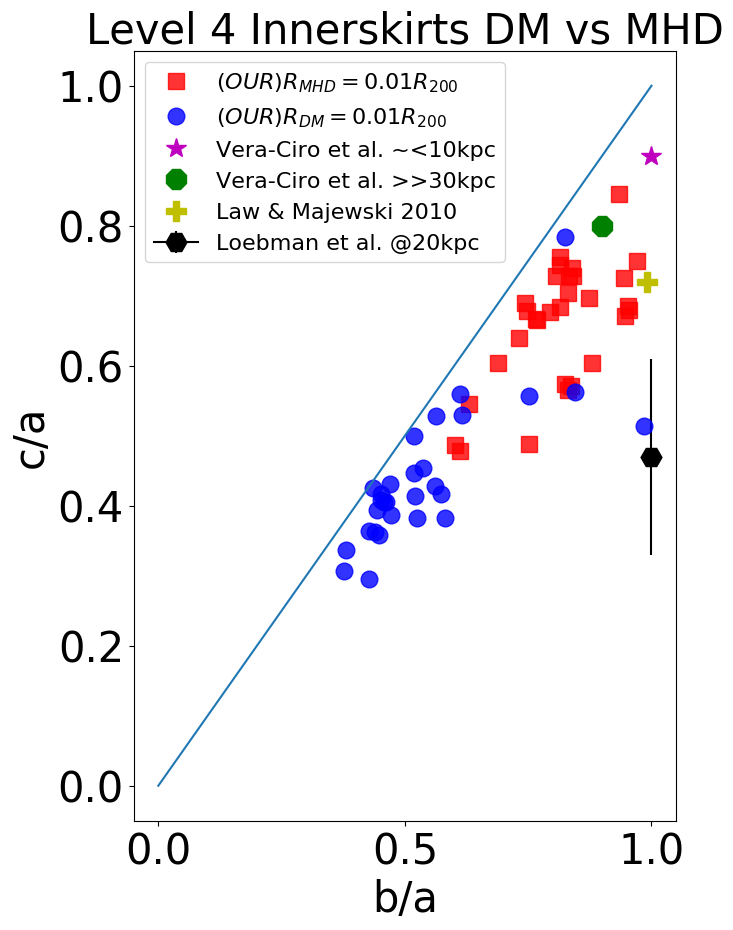
\includegraphics[width=0.7\columnwidth]{./pics/Triaxial_Plane/Triaxiality_Inner_lvl4.png}}
  \hfill
  \subfloat[Level4 MHD Vs DM at outter regions]{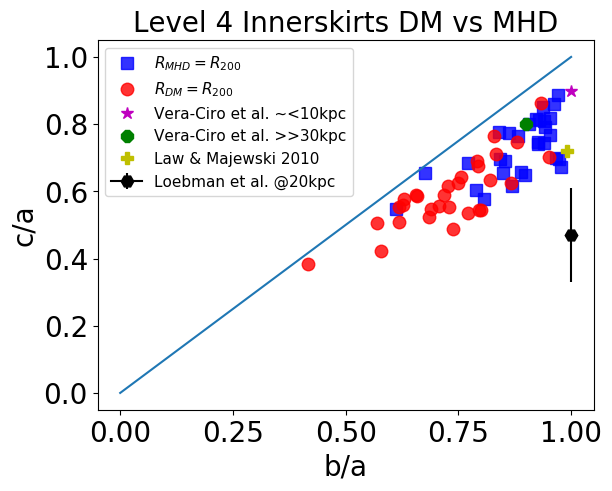
\includegraphics[width=0.7\columnwidth]{./pics/Triaxial_Plane/Triaxiality_Outter_lvl4.png}}
  \hfill
  \caption{General tendence on the triaxial plane $c/a$ Vs $b/a$. Some observational constraints (stars and error-bar point) are plotted alongside our results}
  \label{fig:Triaxiality_Inner_Outer}
\end{figure}


\subsection{The effect of gas on the halo shape}
We have simultaneously corroborated the rounding effect of radius on the halo shape from DM-only and MHD simulations. However, from the parallel presentation of both of the results, it is easily noticeable that there is also a relation of this rounding effect in terms of the presence of matter, which is to be expected \cite{effect of gas}.\\

 Unlike DM, gas collapses and generate disks which are much denser than the DM structures. This amplifies scattering events and, if we apply the same logic, we would expect that the inner regions of the halo are more spherical when there is presence of gas. We expect the same for outter regions but this effect is predicted to be more significant due to the stronger effect of the gravitational potential of gas on the outter shells.\\

For instance, recurring again to the figures \ref{fig:slices}, now comparing the graphics vertically, the rounding effect of visible matter is clear. For a more cuantitative illustration of this, we can reffer to figure \ref{fig:DM_MHD}. \\
\begin{figure}[!ht]
  \centering
  \subfloat[Level4 DM inner Vs outer regions]{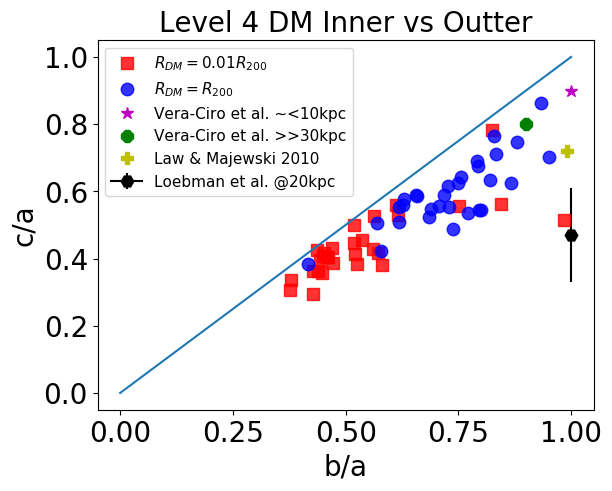
\includegraphics[width=0.7\columnwidth]{./pics/Triaxial_Plane/Triaxiality_DM_lvl4.png}}
  \hfill
  \subfloat[Level4 MHD inner Vs outter regions]{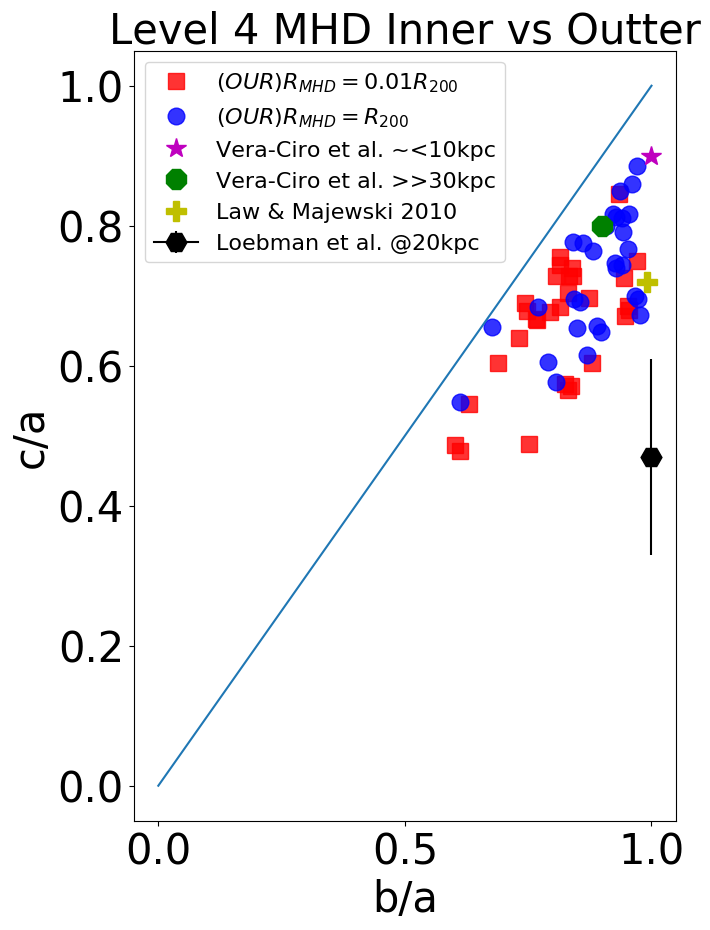
\includegraphics[width=0.7\columnwidth]{./pics/Triaxial_Plane/Triaxiality_MHD_lvl4.png}}
  \hfill
  \caption{General tendence on the triaxial plane $c/a$ Vs $b/a$. Some observational constraints (stars and error-bar point) are plotted alongside our results}
  \label{fig:Triaxiality_DM_MHD}
\end{figure}

Although from previous pictures it is evident that the presence of gas affects the halo shape by rounding it, it is not clear that this effect is amplified for bigger radii. To confirm this, we reccurr again to triaxiality plane on \ref{fig:Triaxiality_DM_MHD}, where this tendency becomes evident.\\


So far, our results are in accordance with previous work on different kinds of simulations. Nonetheless, on the specific case of MW-like galaxy simulations, we have confirmed the expected tendence in an unprecedented statistically significant sample of 30 galaxies form Auriga, compared to the 4-sample galaxies from the previous state-of-the art DM-only Aquarius simulations. Moreover, we confirmed that these results are sustained for the specific case of novel MHD MW-like galaxy simulations.\\

\section{Historical shape}
Taking into account the previously explained model of formation of halos as a qualitative theoretical background that supports our results, it is possible to extend 
its reach not only for refshift 0 predictions but for the analysis of the historical evolution of the halo shape \cite{}.\\

 Recalling that inner shells of the halo are isolated from the gravitational effect of outer shells, the only source of disruption in time of this radial regime are external cosmic structures that perform some torque on them. Outter shells must feel this source of deformation too in addition to the effect of scattering from the inner gravitational potential. Consequently, we expect a systematic change on the halo shape with time, which becomes more significant for bigger radii.\\
 
Major events, like mergers, may completely disturb a galaxy shape and erase any memory of it. However, from $z~1$ onwards, these events are very rare \cite{} and we expect that any source of disruption is weak and is reduced to the previously mentioned factors. These sources of anisotropy and scattering randomize DM particle orbits producing a more spherical version of the halo. \cite{} \\  

\begin{figure}[!ht]
  \centering
  \subfloat[halo 16 DM]{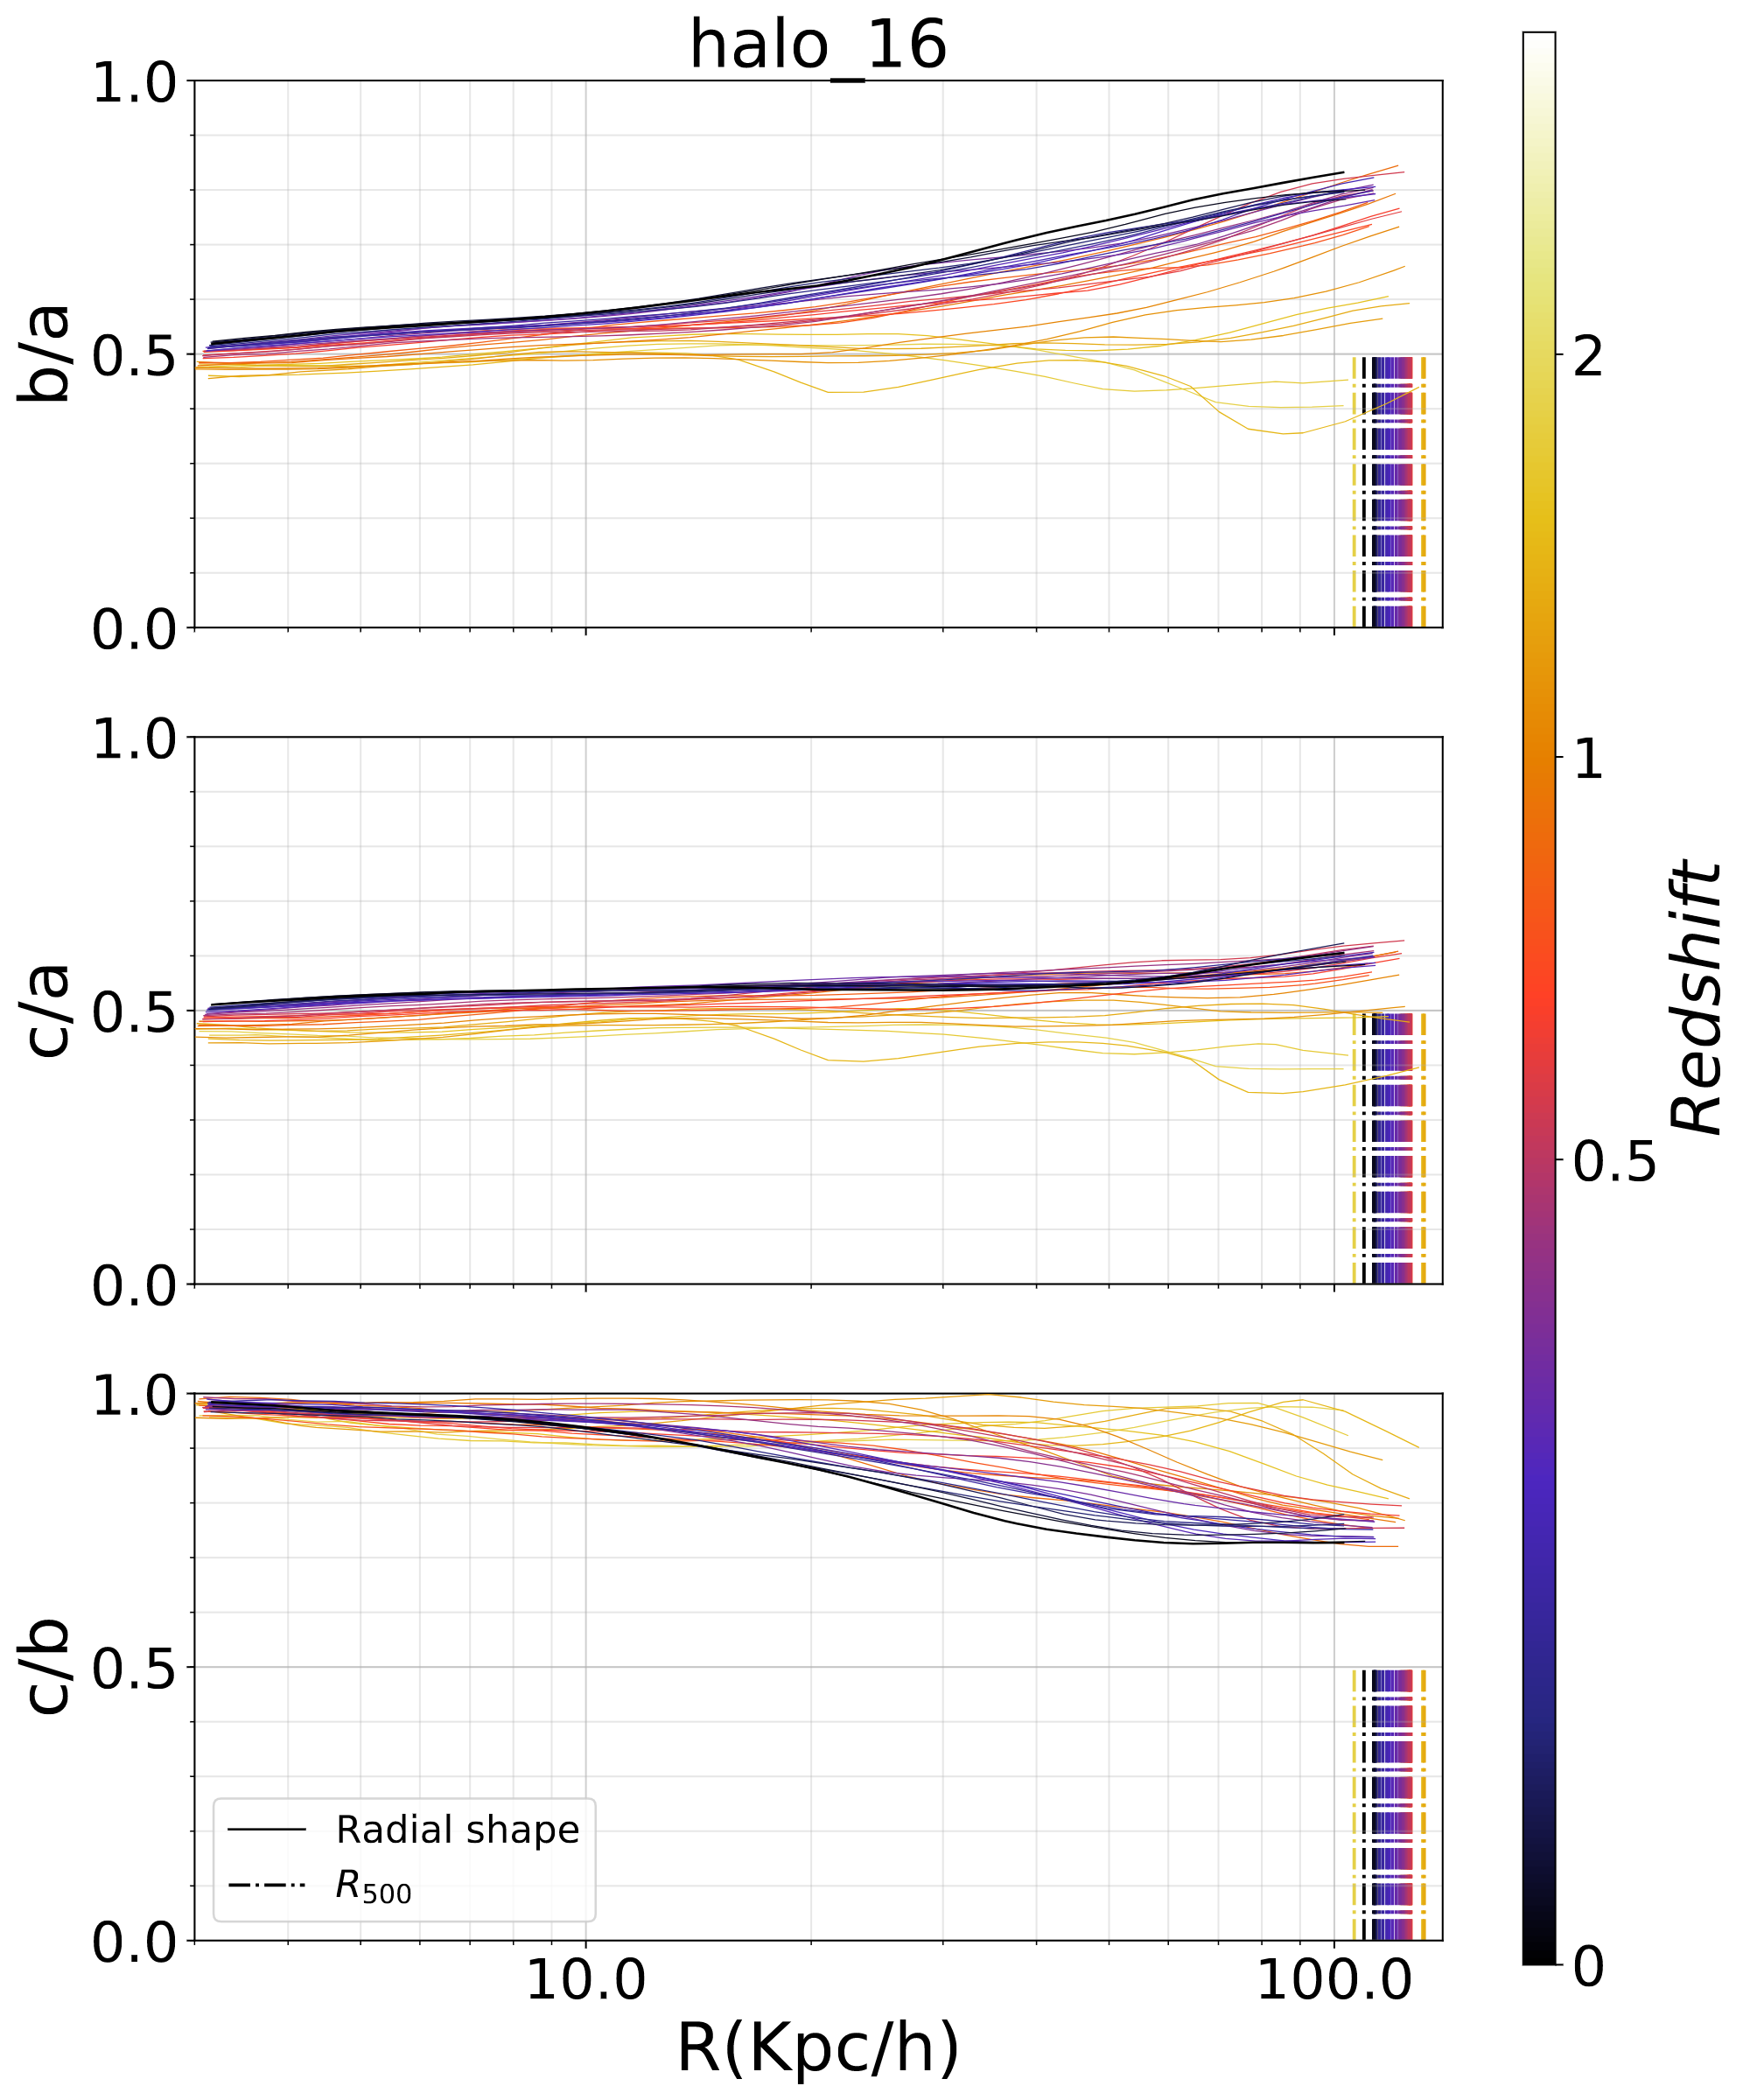
\includegraphics[width=0.7\columnwidth]{./pics/Redshift/halo_16_level3_DM_Z.png}}
  \hfill
  \subfloat[halo 16 MHD]{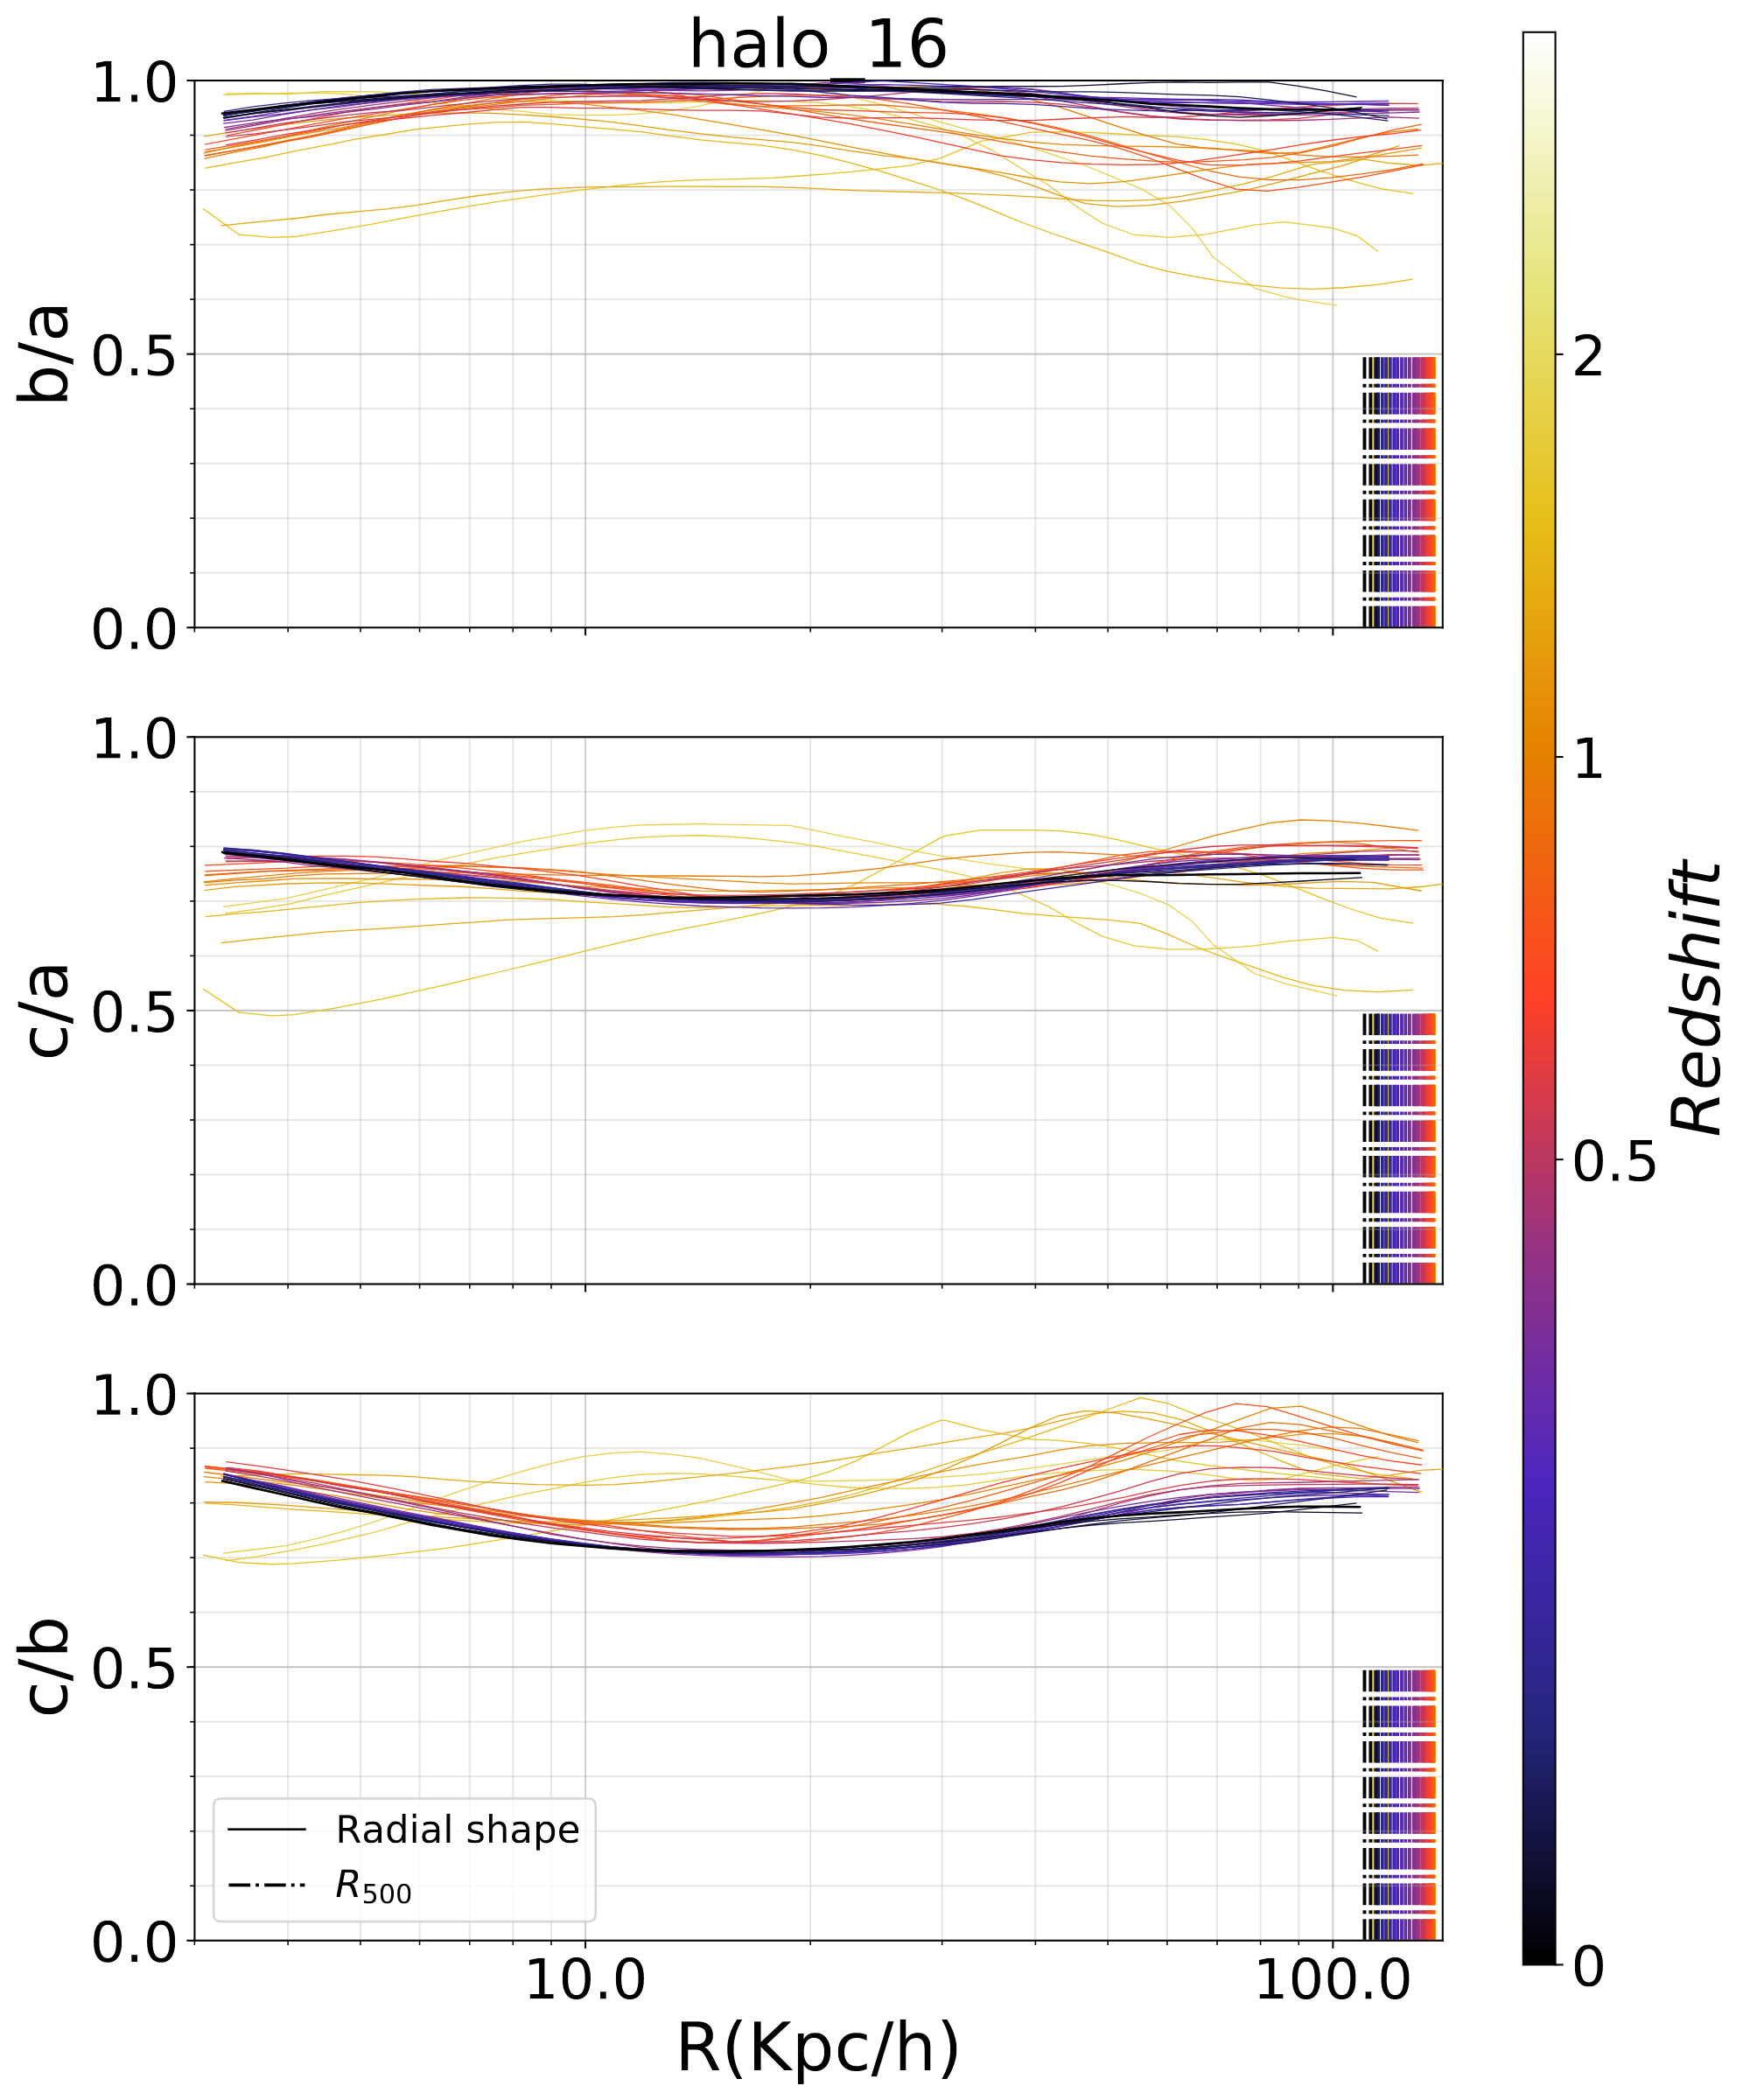
\includegraphics[width=0.7\columnwidth]{./pics/Redshift/halo_16_level3_MHD_Z.png}}
  \caption{Example of historic shape conservation in comoving coordinates.}
  \label{fig:RedshiftGood}
\end{figure}

In figures \ref{fig:RedshiftGood} we present the evolution of the radial profile of the shape of a halo that managed to conserve its integrity until $z~2$. In this case, we present our results in terms of the comoving coordinates to make these profiles comparable. The halo becomes sistematically more spherical as it evolves in time, being this effect more relevant for $r>50Kpc$.\\

In figures \label{fig:RedshiftDMbad} we present a very special case of a halo that was perturbed at some time around $z=0.5$. It is specially evident because of the discontinuity caused in the radial profile and the large differences in the different virial radii. \\  


\begin{figure}[!ht]
  \centering
  \subfloat[halo 21 DM]{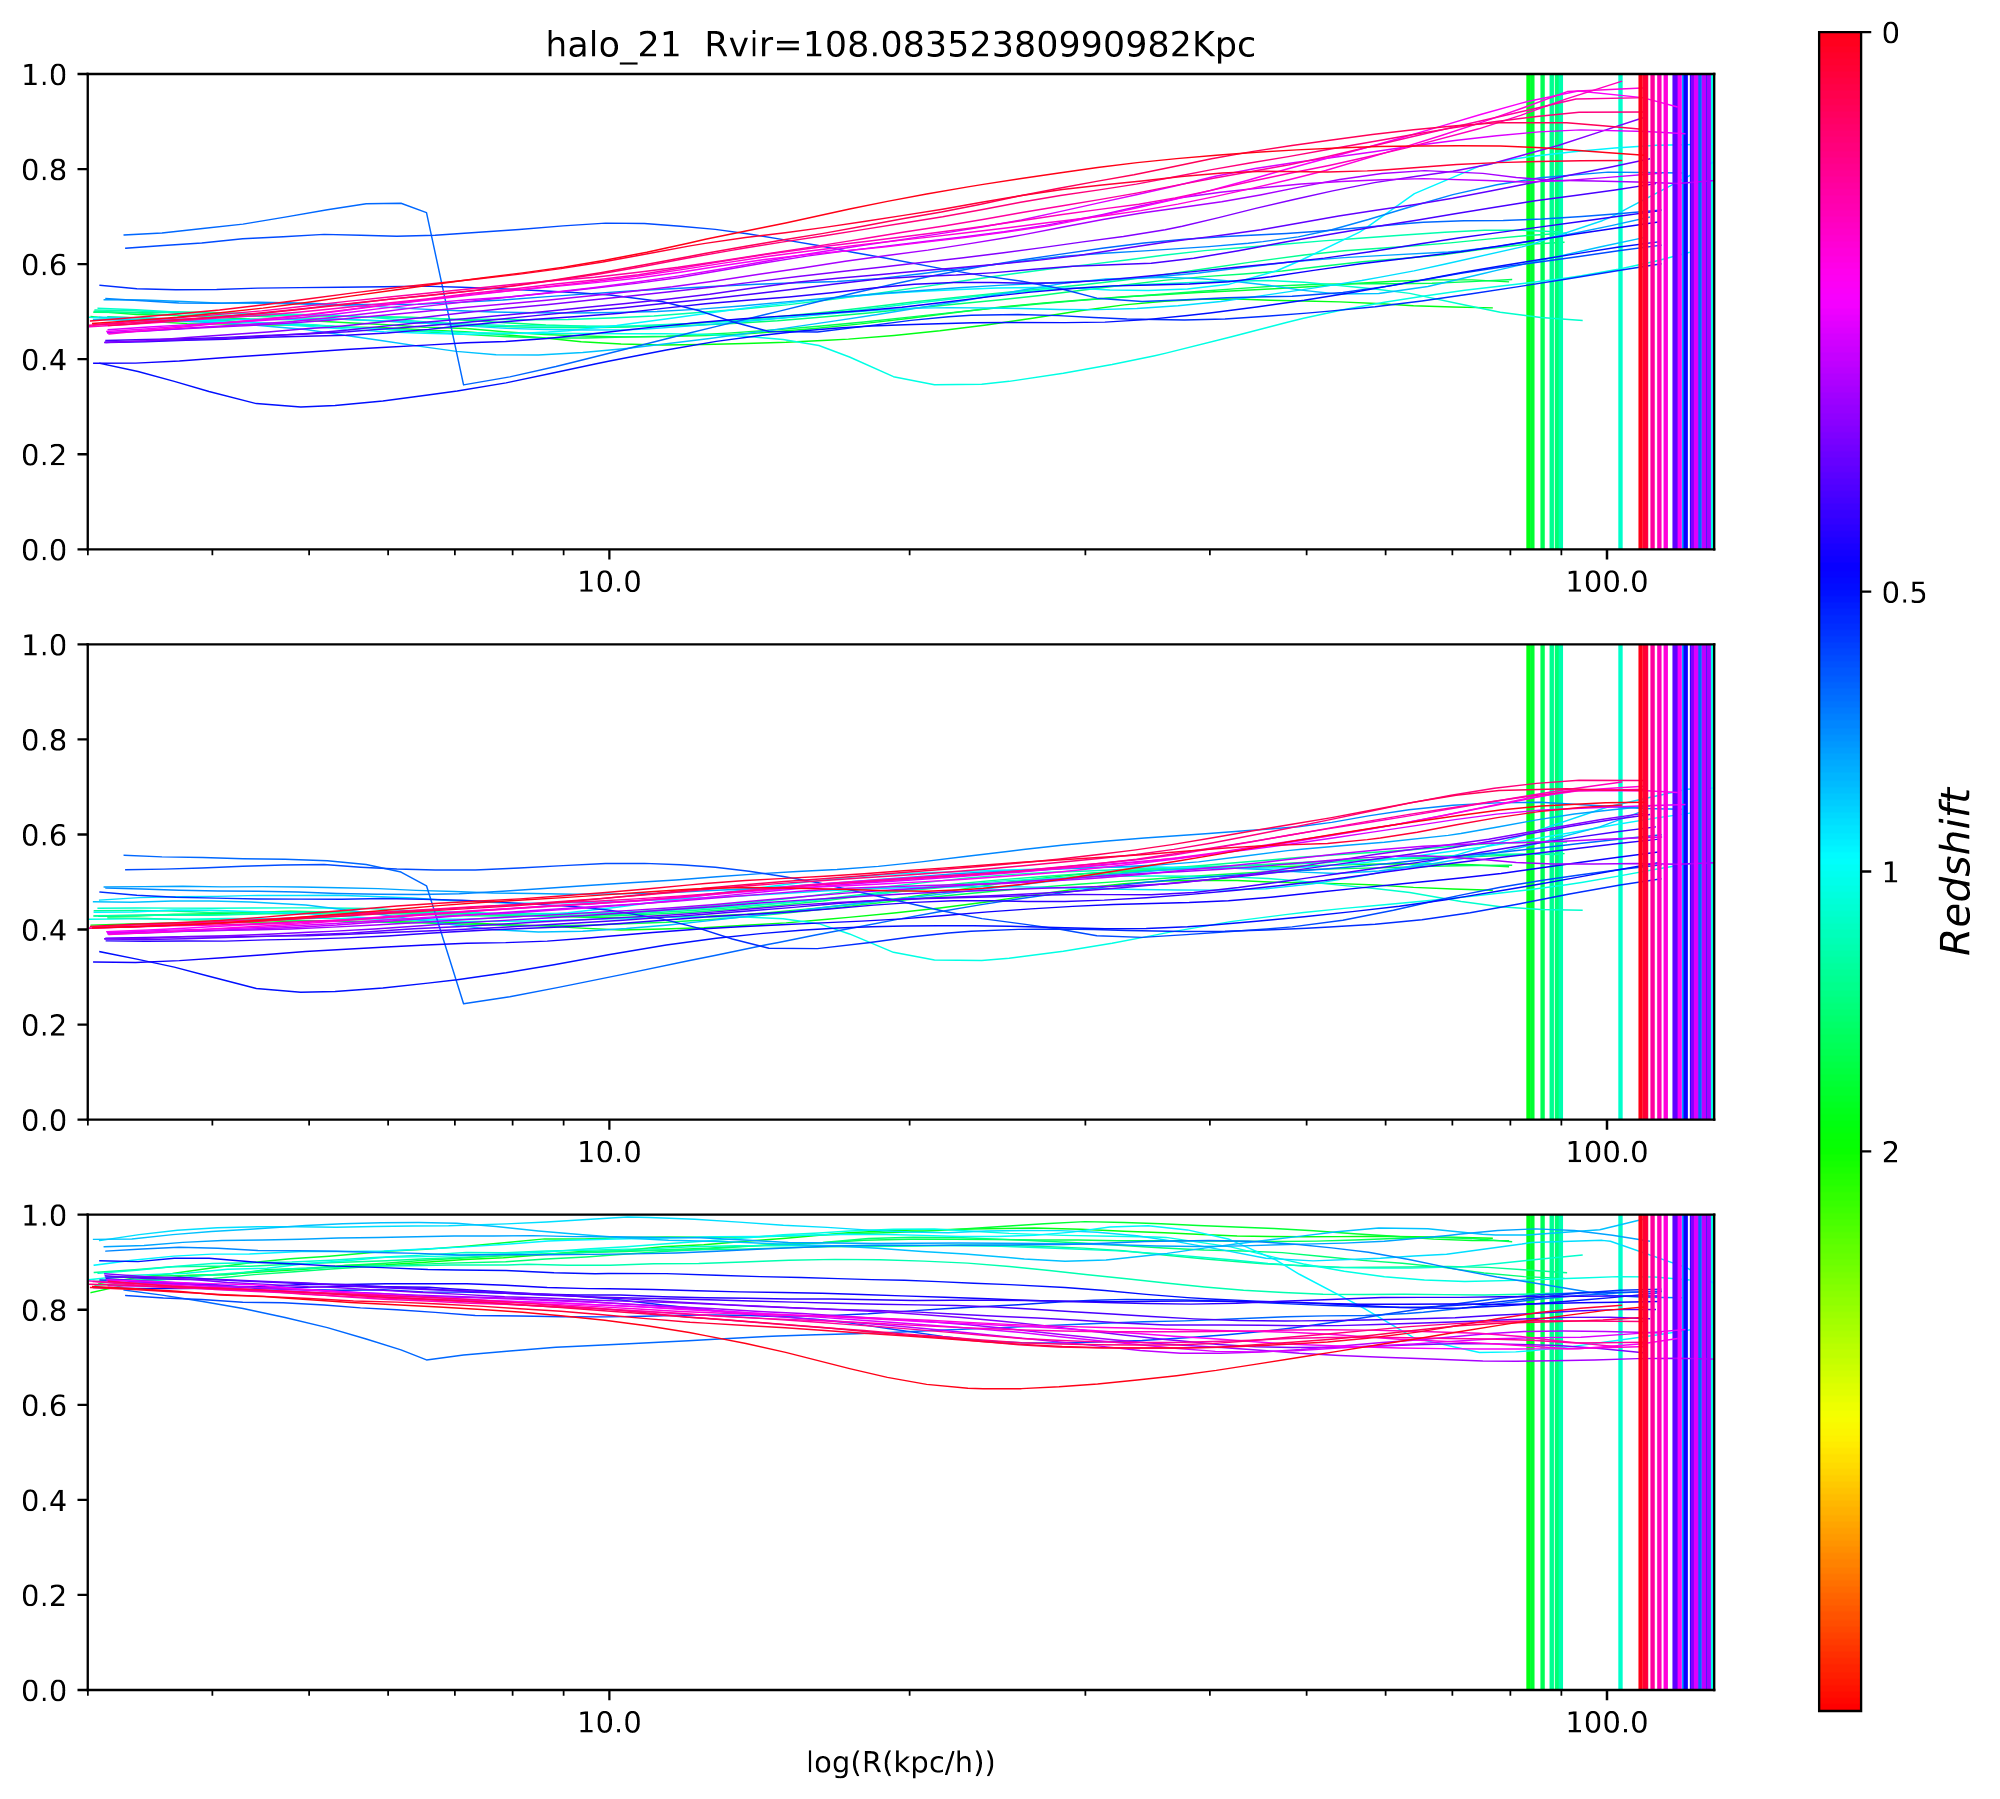
\includegraphics[width=0.7\columnwidth]{./pics/Redshift/halo_21_level3_DM_Z.png}}
  \hfill
  \subfloat[halo 21 MHD]{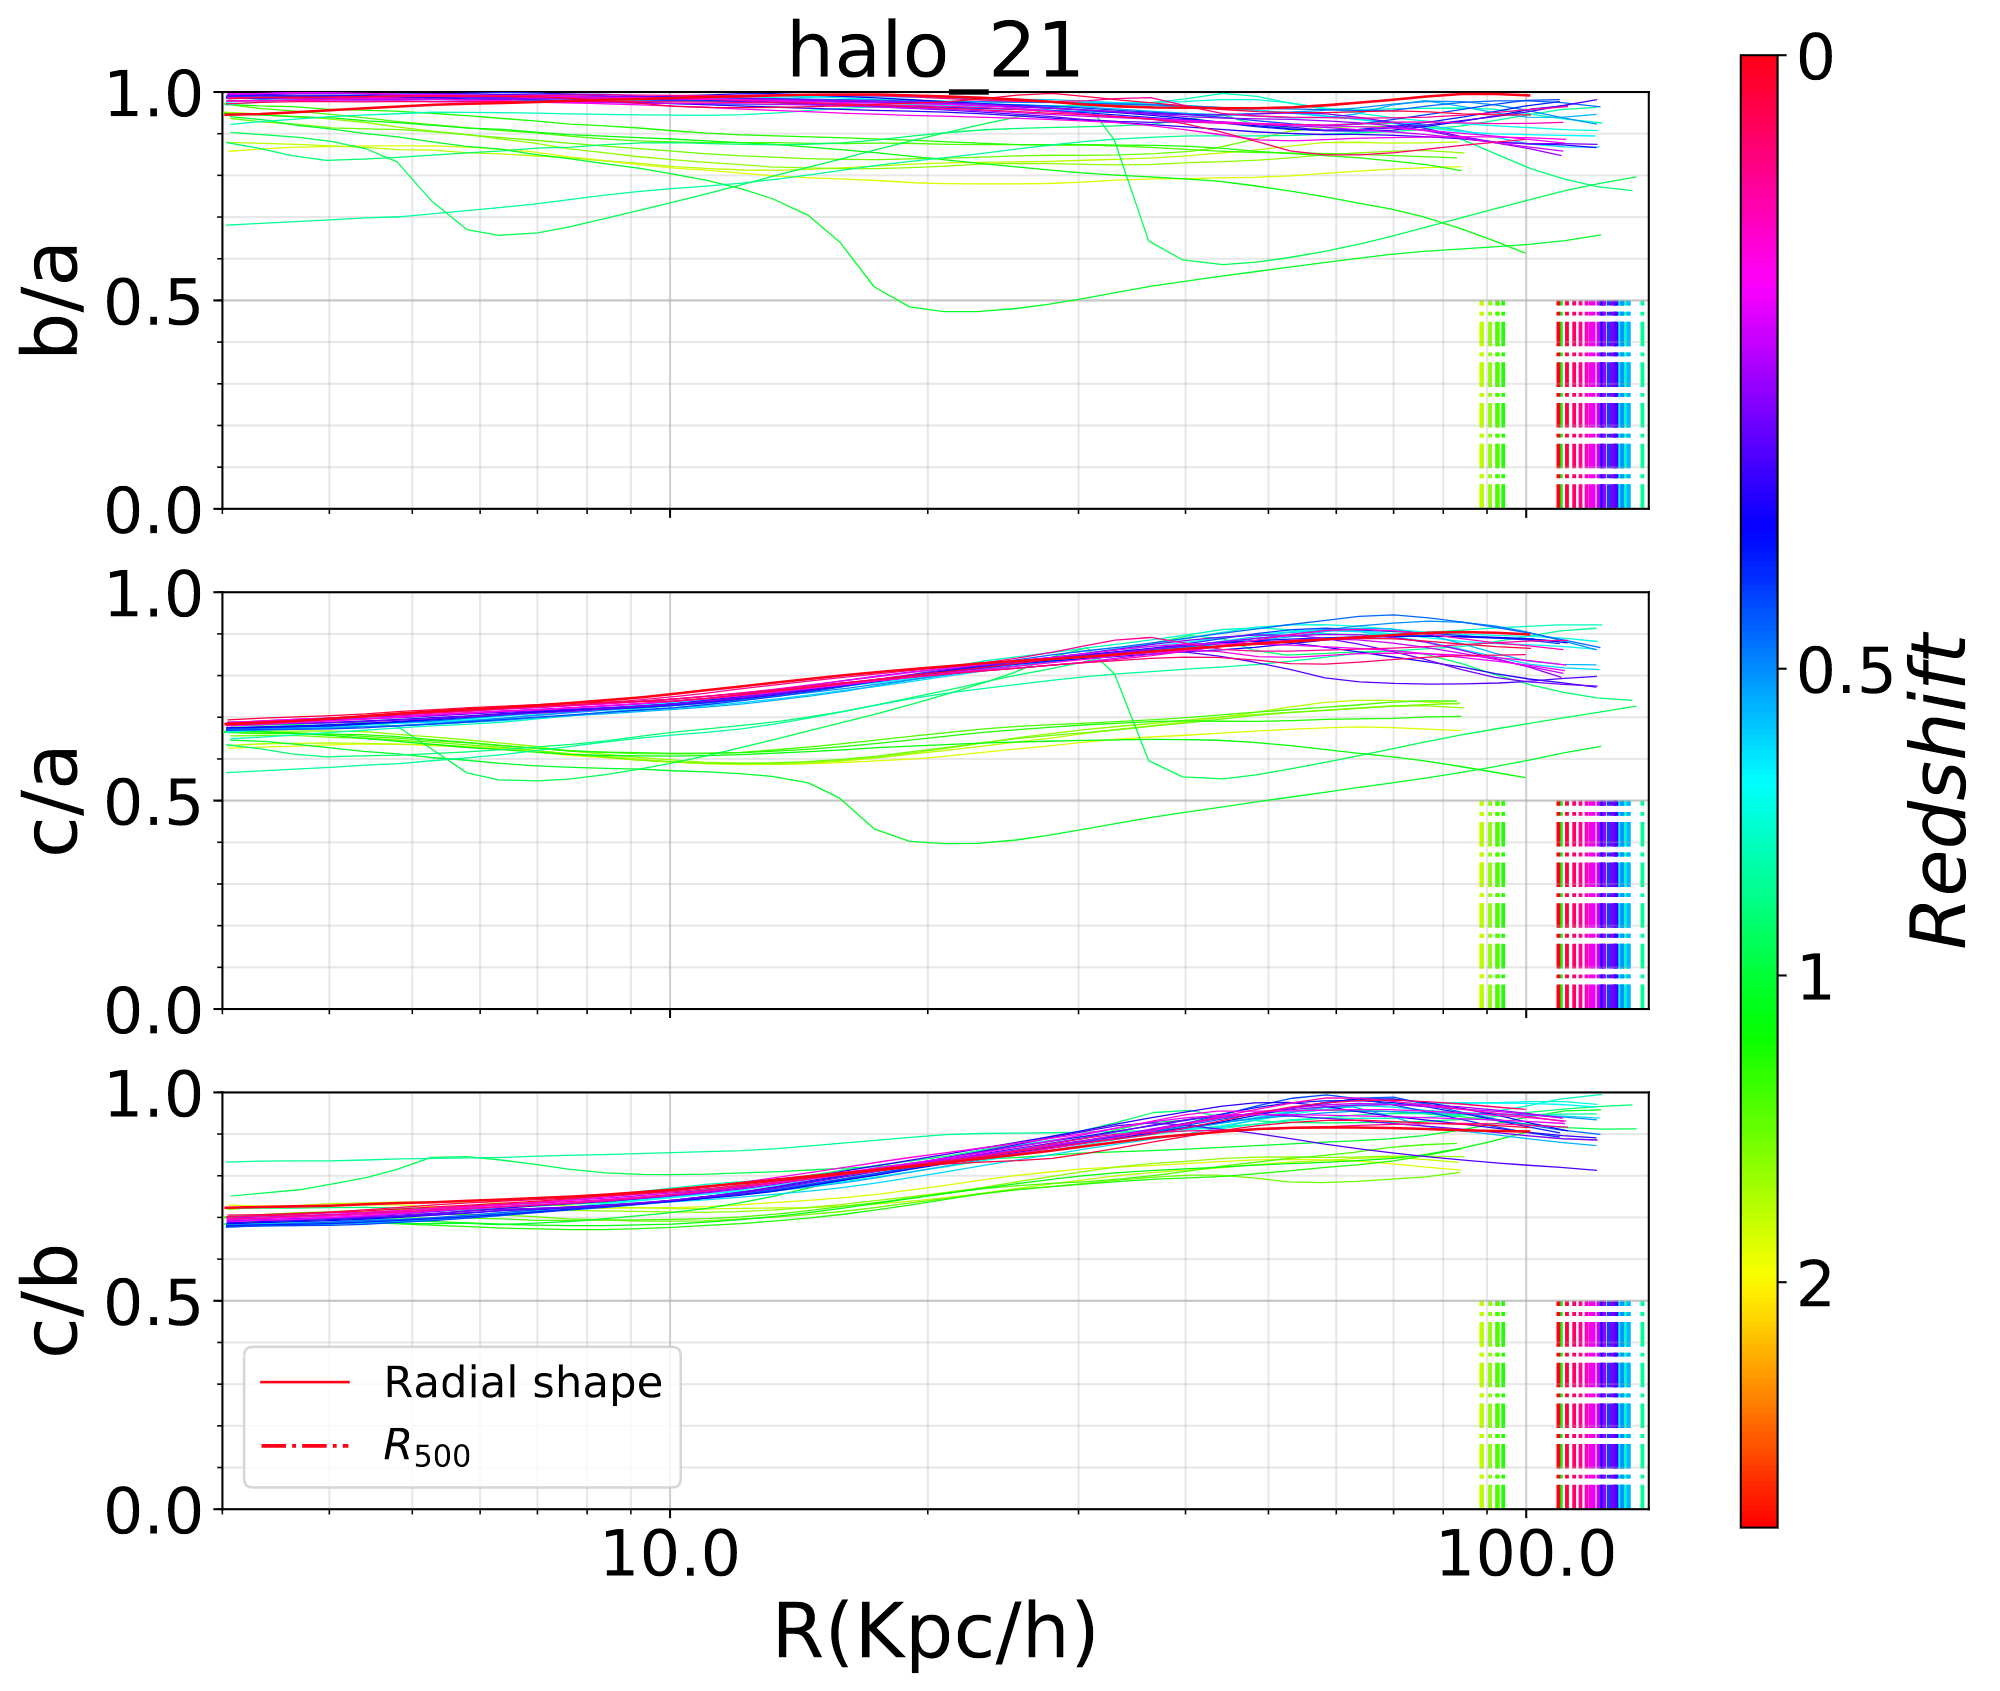
\includegraphics[width=0.7\columnwidth]{./pics/Redshift/halo_21_level3_MHD_Z.png}}
  \caption{Example of historic shape disruption in comoving coordinates. The consistency between MHD and DM implies some major-event like a close merger or a collision. The non-continuous red line corresponds to a very close moment of this merging event, which is amplified in MHD.}
  \label{fig:RedshiftBad}
\end{figure}

Now, these results compare radial profiles in comoving coordinates, but in real life we have physical coordinates. In this order of ideas, we can state this conservation of the shape (obviating the rounding effect) in terms of physical coordinates.\\

In this case, let us consider a constant physical radius $R$ at which we are going to perform our measurements at different redshifts. For practical purposes let us take, for example, the virial radius at $z=0$. Then, if we want to obtain the shape at higher redshifts, it is necessary to obtain the corresponding physical radius using the scaling factor $a$. As the universe is expanding, we are effectively sampling the shape for smaller radii at higher redshifts. Taking into account that the halo shape is well conserved in time, we expect that studying the historical profile of the shape at a certain constant physical radius is nearly equivalent to studying the radial profile of the same halo at the present time. \\

To illustrate this, in figures \ref{fig:RedshiftDMTriax16,fig:RedshiftDMTriax21} we present the historical and radial profiles of the previously analyzed halo shapes. For the halo that maintained a consistent shape during time, there is a clear correlation between the historical and radial profiles, both clearly tending to more spherical shapes at lower redshifts and bigger radii. In the case of the halo that had a major disrupting event, this correlation is not clear, however, a difuse tendence to rounder shapes still remains.\\  

\begin{verbatim}
\begin{figure}[!ht]
  \centering
  \subfloat[halo 16 MHD]{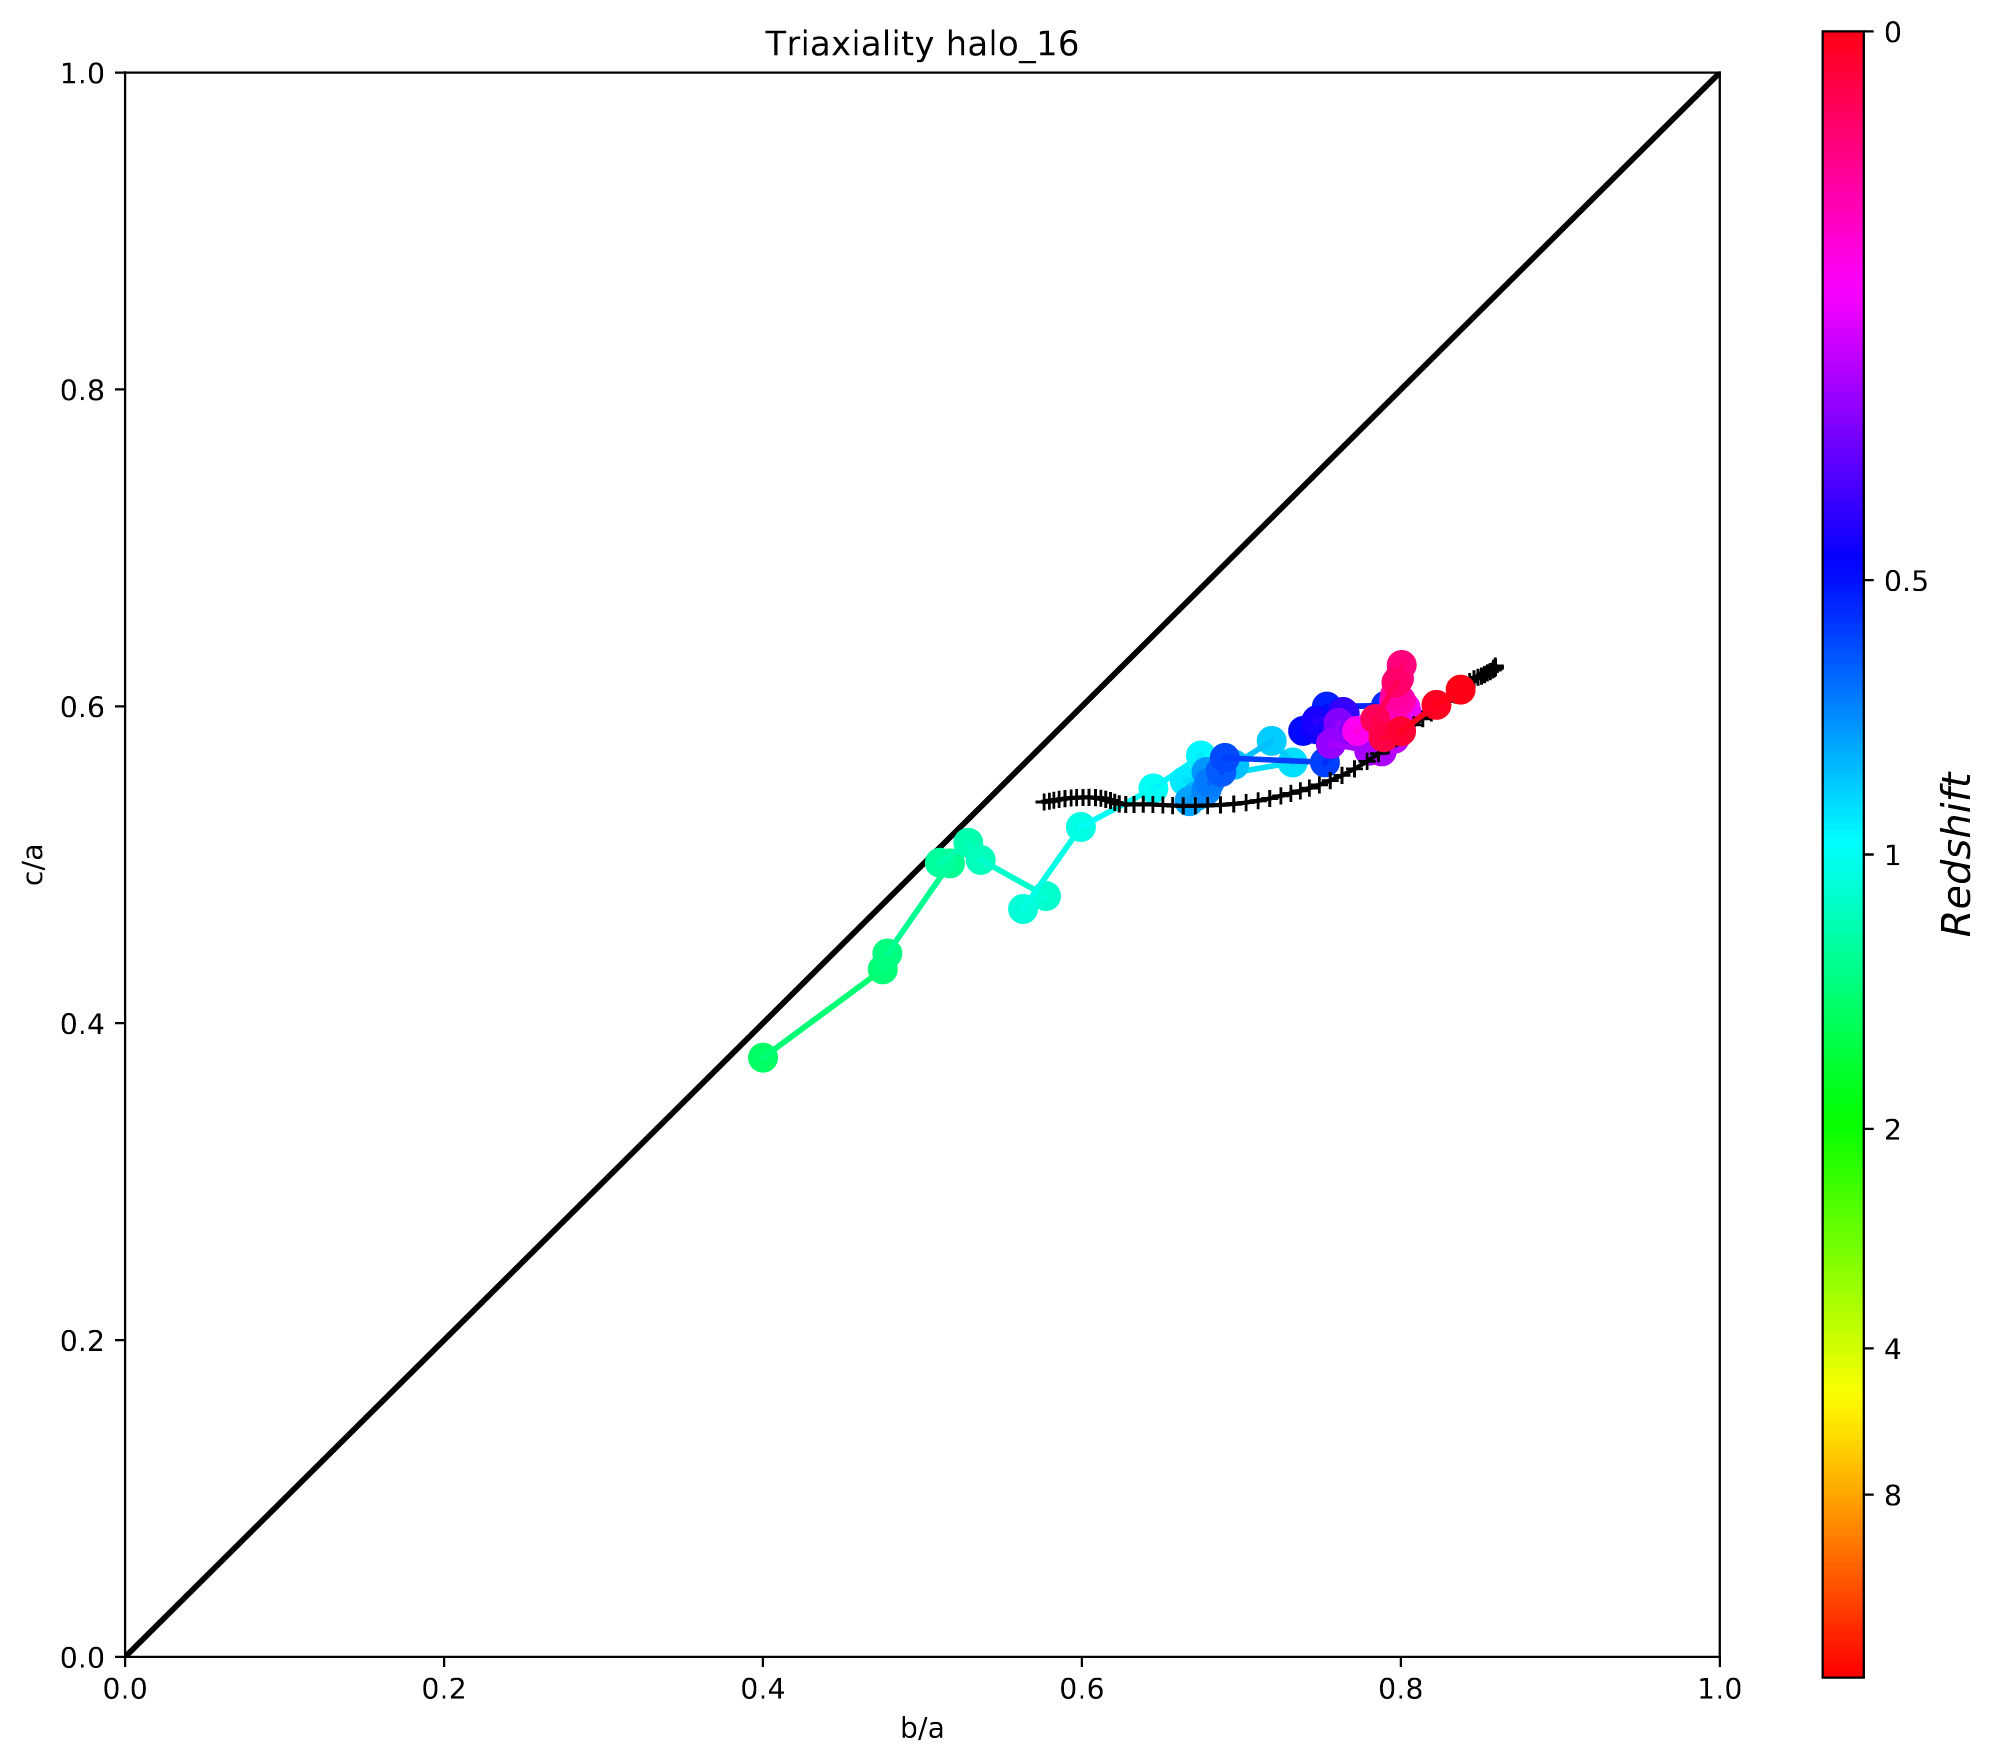
\includegraphics[width=0.7\columnwidth]{./pics/Redshift/halo_16_level3_MHD_Z_Triax.png}\label{fig:RedshiftDMTriax16}}
  \hfill
  \subfloat[halo 21 MHD]{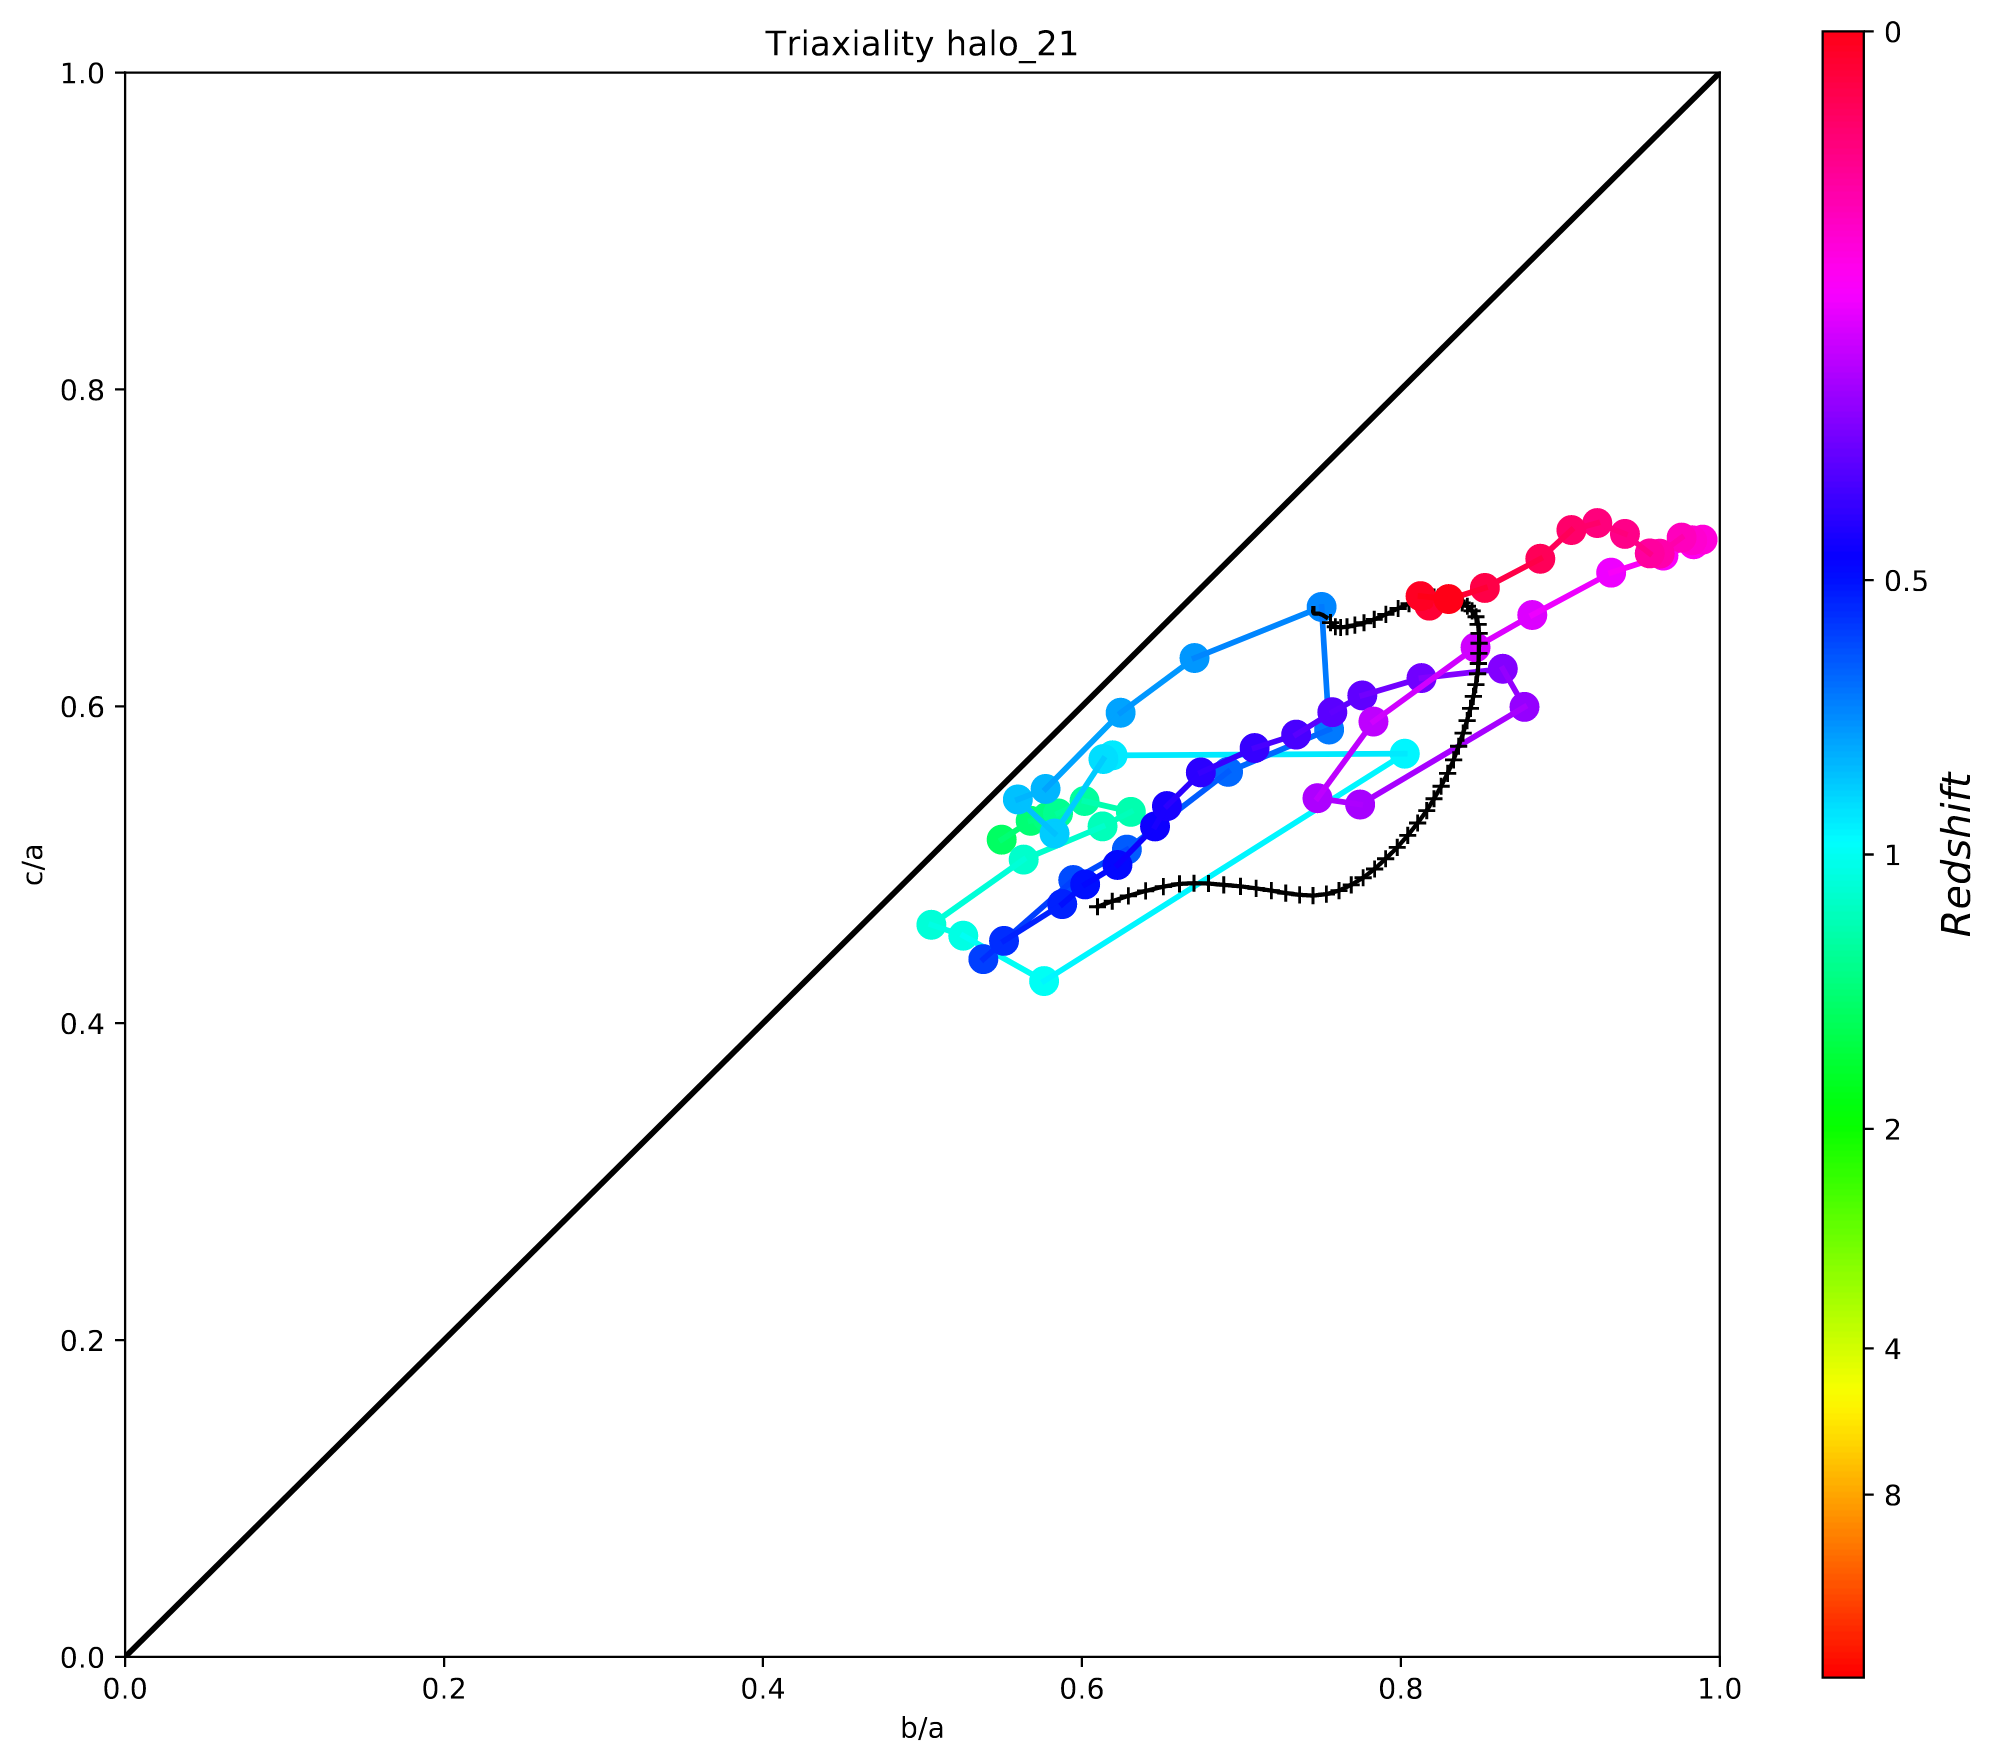
\includegraphics[width=0.7\columnwidth]{./pics/Redshift/halo_21_level3_MHD_Z_Triax.png}\label{fig:RedshiftDMTriax21}}
  \caption{Historic shape Vs radial shape on the Triaxiality plane. The black line represents the radial profile at redshift 0. The colored connected dots represent the shape measured at the virial radius (physical coordinates) at a certain redshift (color)}
\end{figure}
\end{verbatim}







 
